% ============================================================================
% Article scientifique — Scoring de crédit PME en RDC via XGBoost-Boruta-GHM
% ============================================================================
\documentclass[12pt, a4paper, twocolumn]{article}

% --- Encodage et langue ---
\usepackage[utf8]{inputenc}
\usepackage[T1]{fontenc}
\usepackage[french]{babel}
\usepackage{microtype}

% --- Mise en page ---
\usepackage[top=2.5cm, bottom=2.5cm, left=2cm, right=2cm]{geometry}
\usepackage{setspace}
% \onehalfspacing  % disabled for two-column layout

% --- Mathématiques ---
\usepackage{amsmath, amssymb, amsfonts}

% --- Graphiques et figures ---
\usepackage{graphicx}
\graphicspath{{figures/}}
\usepackage{float}
\usepackage[labelfont=bf, font=small]{caption}
\usepackage{subcaption}

% --- Tableaux ---
\usepackage{booktabs}
\usepackage{array}
\usepackage{multirow}
\usepackage{tabularx}
\usepackage{longtable}

% --- Couleurs et liens ---
\usepackage[dvipsnames]{xcolor}
\usepackage[colorlinks=true, linkcolor=MidnightBlue, citecolor=OliveGreen, urlcolor=BrickRed]{hyperref}

% --- Bibliographie ---
\usepackage[numbers, sort&compress]{natbib}

% --- Code et listings ---
\usepackage{listings}
\lstset{
  basicstyle=\small\ttfamily,
  frame=single,
  breaklines=true,
  columns=fullflexible,
}

% --- Divers ---
\usepackage{enumitem}
\usepackage{fancyhdr}
\usepackage{titlesec}
\usepackage[title]{appendix}
\usepackage{balance}

% --- En-tête / pied de page ---
\pagestyle{fancy}
\fancyhf{}
\fancyhead[L]{\small\textit{Scoring PME -- RDC}}
\fancyhead[R]{\small\textit{XGBoost-B-GHM + CET via Wanzo}}
\fancyfoot[C]{\thepage}
\renewcommand{\headrulewidth}{0.4pt}

% ============================================================================
\title{%
  \textbf{Utilisation de données synthétiques et d'intelligence artificielle pour la conception d'un modèle de prédiction de défauts de paiement des PME en République Démocratique du Congo} \\[0.8em]
  \large Approche XGBoost-Boruta-GHM intégrant le Contexte Économique Territorial via l'ERP Wanzo
}

\author{
  Jacques NDAVARO\textsuperscript{1} \and David KRAME\textsuperscript{1} \\[0.3em]
  \small\textsuperscript{1} Centre de Recherche et d'Expertise Scientifique (CRES) \\
  \small \texttt{jacquesndav@ikiotahub.com} \quad \texttt{david.krame@aims-cameroon.org}
}

\date{Mars 2026}

% ============================================================================
\begin{document}
\twocolumn[
  \begin{@twocolumnfalse}
    \maketitle
    \begin{abstract}
La République Démocratique du Congo (RDC) fait face à un défi structurel d'inclusion financière~: plus de 70\,\% de l'activité économique des PME s'effectue hors des circuits bancaires formels. Les modèles classiques de scoring, développés sur des données nord-américaines et européennes, souffrent d'un \textbf{biais systémique de représentativité} inadapté au contexte africain.

Cet article présente une méthodologie articulée autour de trois axes~: (1)~un \textbf{état de l'art des méthodes de génération de données synthétiques} tabulaires, des approches paramétriques (SDV, copules) aux modèles d'IA générative (CTGAN \cite{xu2019ctgan}, TabDDPM \cite{kotelnikov2023}, GReaT \cite{borisov2023}), justifiant le choix d'une approche paramétrique guidée par l'expertise~; (2)~la construction d'un modèle \textbf{XGBoost-Boruta-GHM} \cite{xia2024} intégrant données transactionnelles ERP Wanzo, un cadre original de \textbf{Contexte Économique Territorial (CET)} capturant les spécificités de l'économie informelle congolaise, et des données alternatives~; (3)~une analyse des \textbf{biais des modèles de scoring vis-à-vis de l'Afrique} et une réponse «~\textit{by design}~» via le CET, scoring natif congolais plutôt que modèle occidental adapté.

Le modèle, entraîné sur 5\,000 PME synthétiques (taux de défaut~: 13\,\%), atteint une \textbf{AUC-ROC de 0,767} et une précision de 87,4\,\%. L'analyse SHAP confirme que les ratios de trésorerie, les variables comportementales et les scores CET (15\,\% des variables retenues par Boruta) constituent les facteurs les plus discriminants. Un scoring sur échelle 300--850 permet une classification en cinq catégories de risque, démontrant la faisabilité d'un scoring contextualisé liant théorie de l'information et inclusion financière via la plateforme Wanzo.

\medskip
\noindent\textbf{Mots-clés~:} Credit scoring, PME, données synthétiques, XGBoost, Boruta, GHM, CTGAN, biais algorithmique, contexte économique territorial, inclusion financière, RDC, ERP, IA générative.
    \end{abstract}
    \vspace{1em}
  \end{@twocolumnfalse}
]

% ============================================================================
\section{Introduction}
\label{sec:introduction}

% ----------------------------------------------------------------------------
\subsection{Contexte~: l'inclusion financière en RDC}
\label{subsec:contexte}

La République Démocratique du Congo, avec ses 100 millions d'habitants et un tissu de micro, petites et moyennes entreprises (MPME) représentant la colonne vertébrale de son économie, constitue un terrain où la problématique de l'inclusion financière se pose avec une acuité particulière. Le secteur informel, estimé à plus de 70\,\% du PIB, opère largement en dehors des circuits bancaires formels \cite{bcc2023}. Les transactions s'effectuent majoritairement en espèces (${\sim}80\,\%$), complétées par le mobile money (${\sim}17\,\%$) et les virements bancaires (${\sim}3\,\%$), une structure de paiement qui rend les méthodes classiques d'évaluation de crédit, fondées sur l'historique bancaire, profondément inadéquates.

Cette réalité a motivé la création de plusieurs initiatives institutionnelles visant à combler le fossé financier~:

\begin{itemize}[leftmargin=*]
  \item \textbf{Le Fonds pour la Promotion de la Microfinance (FPM)}, créé en 2010 sous forme d'ASBL puis transformé en société anonyme en 2014, représente le principal instrument d'appui à l'inclusion financière des MPME en RDC. Avec un portefeuille de 31,4 millions USD et 569 projets financés à travers 40 partenaires (PAIDEK~SA, TUJENGE PAMOJA~SA, SMICO~SA, BAOBAB RDC, ADVANS CONGO, EQUITY BCDC, Procfin~SA), le FPM agit par trois mécanismes~: l'assistance technique aux institutions de microfinance, le refinancement et la garantie de portefeuille \cite{fpm2024}. Le programme d'éducation financière, développé en partenariat avec VISA, et la donation de 20 millions EUR de la KFW témoignent de l'envergure de cet effort.

  \item \textbf{Le projet TRANSFORME} (Projet d'autonomisation des femmes entrepreneures et mise à niveau des PME pour la transformation économique et l'emploi), financé par la Banque Mondiale et succédant au PADMPME, cible spécifiquement la mise à niveau des PME congolaises et l'autonomisation des femmes entrepreneures. Coordonné par Alexis Mangala sous la tutelle du Ministère de l'Industrie, TRANSFORME constitue un levier majeur pour la formalisation et la compétitivité des PME \cite{transforme2024}. Le FPM~SA opère également le Fonds GPP (Garantie de Portefeuille de Prêts) via TRANSFORME avec une enveloppe de 20 millions USD.

  \item \textbf{Le FOGEC} (Fonds de Garantie de l'Entrepreneuriat au Congo), sous la direction de Laurent Munzemba, a financé 328 projets dans 16 provinces pour un montant global de 3,2 millions USD, générant 2\,700 emplois (1\,150 directs et 1\,550 indirects). Ses produits innovants (Vijana pour les jeunes entrepreneurs, Tombola nkita nayo, initiatives de crowdfunding et business angels) illustrent une approche adaptée au contexte congolais \cite{fogec2024}.
\end{itemize}

% ----------------------------------------------------------------------------
\subsection{Problématique~: l'absence de données structurées}
\label{subsec:problematique}

Le paradoxe central de l'inclusion financière en RDC réside dans un cercle vicieux informationnel~: les PME n'accèdent pas au crédit faute d'historique financier vérifiable, et elles ne constituent pas d'historique précisément parce qu'elles sont exclues du système formel. Comme le souligne Guérin \cite{guerin2015} (p.~102--106), «~le crédit seul est insuffisant~; c'est la capacité d'absorption locale et l'accès aux marchés qui déterminent le succès de l'inclusion financière~».

Ce constat implique la nécessité d'une approche radicalement différente~:

\begin{enumerate}[leftmargin=*]
  \item \textbf{Générer des données synthétiques} calibrées sur les réalités économiques congolaises lorsque les données historiques font défaut~;
  \item \textbf{Intégrer des sources de données alternatives} allant au-delà de la comptabilité formelle~: réseaux communautaires, réputation locale, comportement de paiement mobile~;
  \item \textbf{Contextualiser les modèles prédictifs} en développant un cadre analytique spécifique au \textbf{Contexte Économique Territorial (CET)} de la RDC.
\end{enumerate}

% ----------------------------------------------------------------------------
\subsection{Contribution et plan de l'article}
\label{subsec:contribution}

Notre contribution est quadruple~:

\begin{itemize}[leftmargin=*]
  \item \textbf{Méthodologique}~: nous proposons un processus rigoureux de génération de données synthétiques pour le scoring de crédit PME, situé dans l'état de l'art des méthodes de génération (paramétrique, CTGAN, TabDDPM, GReaT), validé par des méthodes d'intelligence artificielle et aligné sur les meilleures pratiques académiques \cite{xia2024, nguyen2020}. Nous définissons une feuille de route d'intégration progressive de l'IA générative conditionnée par la collecte de données réelles~;
  \item \textbf{Critique}~: nous analysons les \textbf{biais des modèles de scoring vis-à-vis de l'Afrique et de la RDC} (biais de données d'entraînement, de variables, d'échantillonnage) et proposons un scoring «~\textit{by design}~» natif congolais plutôt qu'un modèle occidental adapté~;
  \item \textbf{Théorique}~: nous introduisons le concept de \textbf{Contexte Économique Territorial (CET)}, un cadre d'analyse intégrant les spécificités de l'économie informelle congolaise dans les modèles prédictifs~;
  \item \textbf{Appliquée}~: nous démontrons comment la plateforme ERP Wanzo, en tant qu'outil de collecte et de structuration de données transactionnelles PME, peut servir de pont entre les initiatives existantes (FPM, TRANSFORME, FOGEC) et les modèles prédictifs fondés sur la théorie de l'information.
\end{itemize}

L'article est organisé comme suit~: la section~\ref{sec:litterature} présente la revue de littérature (scoring IA, données alternatives, microfinance, état de l'art des données synthétiques, biais des modèles en Afrique, théorie de l'information)~; la section~\ref{sec:methodologie} détaille la méthodologie de génération de données et de modélisation~; la section~\ref{sec:resultats} expose les résultats et leur interprétation graphique~; la section~\ref{sec:discussion} discute les implications pour l'inclusion financière et la feuille de route d'intégration de l'IA générative~; la section~\ref{sec:conclusion} conclut.

% ============================================================================
\section{Revue de littérature}
\label{sec:litterature}

% ----------------------------------------------------------------------------
\subsection{Scoring de crédit et intelligence artificielle}
\label{subsec:scoring_ia}

L'évolution du scoring de crédit a connu trois phases distinctes~: les modèles statistiques classiques (régression logistique), les approches de machine learning (random forest, gradient boosting), et les architectures hybrides intégrant sélection de variables et fonctions de perte adaptatives.

\textbf{Xia et al.}~\cite{xia2024}, dans leur article publié dans \textit{MDPI Systems} (Vol.~12, n°7, p.~254), proposent le modèle \textbf{XGBoost-B-GHM} combinant la sélection de variables par l'algorithme Boruta avec une fonction de perte GHM (\textit{Gradient Harmonizing Mechanism}). Leur approche résout deux problèmes simultanés~: (1)~la sélection automatique des variables pertinentes parmi un grand nombre de candidats, et (2)~la gestion du déséquilibre de classes inhérent aux données de crédit. Les paramètres optimaux identifiés, $\text{bins}=7$ et $\beta=0{,}65$ pour le GHM, constituent la base de notre implémentation.

\textbf{Nguyen et Sagara}~\cite{nguyen2020}, dans le cadre du \textit{Working Paper n°1111} de l'Asian Development Bank Institute~(ADBI), démontrent que pour les PME, les \textbf{meilleurs prédicteurs de défaut} sont le \textbf{solde de caisse} et les \textbf{flux de décaissement/remboursement}, davantage que les ratios financiers traditionnels. Leur travail établit également la supériorité des méthodes de machine learning sur la régression logistique pour la prédiction de risque de crédit des PME.

% ----------------------------------------------------------------------------
\subsection{Données alternatives et inclusion financière}
\label{subsec:donnees_alt}

La \textbf{Hong Kong Monetary Authority} (HKMA) \cite{hkma} a formalisé un cadre de scoring de crédit alternatif intégrant des sources non traditionnelles~: factures d'utilités (électricité, eau), données de réseaux sociaux, empreinte numérique et comportement de paiement mobile. Ce cadre est particulièrement pertinent pour les marchés émergents où l'historique bancaire est insuffisant.

% ----------------------------------------------------------------------------
\subsection{Microfinance, capital social et économie informelle}
\label{subsec:microfinance}

\textbf{Guérin}~\cite{guerin2015}, dans \textit{La Microfinance et ses Dérives} (Demopolis/IRD), apporte une perspective critique essentielle pour notre modélisation~:

\begin{itemize}[leftmargin=*]
  \item Les \textbf{réseaux sociaux physiques} (parenté, communauté, associations) sont plus déterminants que la présence numérique dans les économies informelles (p.~86)~;
  \item Le \textbf{capital social} détermine l'accès aux ressources et aux marchés (p.~191--192)~;
  \item Il existe une distinction fondamentale entre l'\textbf{auto-emploi de survie} et l'\textbf{accumulation entrepreneuriale}, qui constituent des profils de risque radicalement différents (p.~82)~;
  \item Les \textbf{tontines et associations d'épargne} (AVEC, COOPEC) fonctionnent comme des pratiques financières structurelles, non comme des indicateurs de marginalité (p.~146).
\end{itemize}

Ces observations justifient notre cadre CET qui pondère les réseaux communautaires et la réputation locale comme des facteurs protecteurs du risque de crédit.

% ----------------------------------------------------------------------------
\subsection{Données synthétiques~: état de l'art des méthodes de génération}
\label{subsec:synth}

L'utilisation de données synthétiques pour l'entraînement de modèles de machine learning a connu une accélération rapide au cours de la dernière décennie \cite{bauer2024, lu2023}. Trois facteurs motivent cette adoption croissante~: (1)~la confidentialité des données bancaires, (2)~l'insuffisance de données dans les marchés émergents, et (3)~la nécessité de tester des architectures avant le déploiement sur données réelles. Nous distinguons quatre générations de méthodes, chacune offrant des compromis différents entre fidélité statistique, complexité et coût computationnel.

\subsubsection{Méthodes classiques (statistiques et paramétriques)}
\label{subsubsec:synth_classique}

Les approches les plus anciennes reposent sur l'échantillonnage de distributions paramétriques (Normale, LogNormale, Beta, Dirichlet) ou sur la création de modèles bootstrap. La \textbf{méthode de Rubin} \cite{rubin1993} (données entièrement synthétiques par imputation de modèles bayésiens) constitue le fondement historique. Le \textbf{Synthetic Data Vault (SDV)} \cite{patki2016} formalise cette approche en apprenant la structure probabiliste d'un jeu de données réel via des copules gaussiennes et des modèles bayésiens hiérarchiques.

\textbf{Avantages}~: reproductibilité totale, contrôle fin des distributions, faible coût computationnel, intégration directe de connaissances d'experts.

\textbf{Limites}~: incapacité à capturer les interactions non-linéaires complexes entre variables, distributions conditionnelles multi-modales, ou dépendances de long rang dans les données tabulaires.

\subsubsection{Réseaux adversariaux génératifs (GANs) pour données tabulaires}
\label{subsubsec:synth_gan}

L'adaptation des GANs \cite{goodfellow2014} aux données tabulaires a constitué une avancée majeure. \textbf{CTGAN} \cite{xu2019ctgan}, publié à NeurIPS~2019, résout deux défis spécifiques~: (1)~les distributions multi-modales des colonnes continues via une transformation \textit{mode-specific normalization}, et (2)~le déséquilibre des catégories via un échantillonnage conditionnel (\textit{conditional vector}). Le générateur architecturé en réseau résiduel et le discriminateur entraîné avec PacGAN produisent des échantillons respectant les corrélations marginales et conjointes. \textbf{TVAE} \cite{xu2019ctgan}, variante autoencodeur variationnel du même travail, offre une alternative plus stable au prix d'une moindre diversité.

CTGAN a démontré sa supériorité sur les réseaux bayésiens pour 5 des 8 jeux de données réels testés, mais reste limité pour les données fortement déséquilibrées (ratio classes $>10$:1) et les jeux de données de petite taille ($<500$ observations), cas fréquent en Afrique.

\subsubsection{Modèles de diffusion pour données tabulaires}
\label{subsubsec:synth_diff}

Plus récemment, les modèles de diffusion ont été adaptés aux données tabulaires. \textbf{TabDDPM} \cite{kotelnikov2023}, publié à ICML~2023, applique un processus de débruitage (\textit{denoising diffusion probabilistic model}) aux vecteurs de caractéristiques hétérogènes (continues et discrètes). TabDDPM traite les variables continues par diffusion gaussienne et les variables catégorielles par diffusion multinomiale, puis apprend à inverser le processus de bruit via un réseau MLP conditionné par la classe.

\textbf{Résultat clé}~: TabDDPM surpasse CTGAN et TVAE sur la majorité des benchmarks testés (15 jeux de données), avec une amélioration moyenne de 7\,\% de l'utilité machine learning et une meilleure préservation de la vie privée.

\subsubsection{Grands modèles de langage (LLMs) comme générateurs tabulaires}
\label{subsubsec:synth_llm}

La dernière frontière est l'utilisation de LLMs auto-régressifs pour la génération tabulaire. \textbf{GReaT} (\textit{Generation of Realistic Tabular Data}) \cite{borisov2023} sérialise chaque ligne d'un tableau en une phrase en langage naturel (ex.~: «~\texttt{anciennete\_annees is 7.5, marge\_nette is 0.49, default is 0}~») et fine-tune un modèle GPT-2 sur ces séquences. Le LLM apprend alors la distribution jointe des caractéristiques et peut générer de nouvelles lignes par échantillonnage auto-régressif, avec la possibilité de conditionner sur n'importe quel sous-ensemble de variables.

\textbf{Avantage unique}~: les LLMs capturent naturellement les dépendances complexes entre types de données hétérogènes et peuvent intégrer des connaissances pré-entraînées. De plus, cette approche permet conceptuellement d'injecter des connaissances contextuelles via le prompt, un atout considérable pour des contextes sous-représentés comme la RDC.

\subsubsection{Synthèse comparative et positionnement}
\label{subsubsec:synth_synthese}

\begin{table}[htbp]
\centering
\caption{Comparaison des méthodes de génération de données synthétiques tabulaires.}
\label{tab:synth_comp}
\small
\begin{tabularx}{\columnwidth}{@{}Xcccc@{}}
\toprule
\textbf{Méthode} & \textbf{Corr.} & \textbf{Rareté} & \textbf{Expert} & \textbf{Coût} \\
\midrule
Param./SDV & $\star\star$ & $\star\star\star$ & $\star\star\star$ & $\star$ \\
CTGAN/TVAE & $\star\star\star$ & $\star\star$ & $\star$ & $\star\star$ \\
TabDDPM & $\star\star\star$ & $\star\star$ & $\star$ & $\star\star\star$ \\
GReaT (LLM) & $\star\star\star$ & $\star\star$ & $\star\star$ & $\star\star\star$ \\
\textbf{Notre (param.+CET)} & $\star\star$ & $\star\star\star$ & $\star\star\star$ & $\star$ \\
\bottomrule
\end{tabularx}
\end{table}

Notre approche se situe dans la \textbf{première génération (paramétrique)} mais s'en distingue par l'injection systématique de connaissances d'experts contextuelles (Persona Wanzo, Guérin, ADBI) dans la conception des distributions et du logit de génération. Ce choix est délibéré~: dans un contexte où \textbf{aucune donnée réelle n'existe} pour entraîner un GAN ou fine-tuner un LLM, l'approche paramétrique guidée par l'expertise reste la seule voie viable. Toutefois, dès que des données réelles seront collectées via l'ERP Wanzo, une transition vers les méthodes génératives (CTGAN puis GReaT) permettra d'améliorer la fidélité des données synthétiques (cf.\ Section~\ref{subsec:discuss_ia}).

% ----------------------------------------------------------------------------
\subsection{Biais des modèles de scoring et enjeux africains}
\label{subsec:biais}

\subsubsection{Le problème fondamental de la représentativité}
\label{subsubsec:biais_represent}

Les modèles dominants de scoring de crédit (FICO Score, VantageScore, modèles bancaires internes) ont été développés sur des données nord-américaines et européennes. Leur transposition directe en Afrique pose un problème fondamental de \textbf{biais de représentativité}~: les distributions de revenus, les structures familiales, les modes de paiement et les dynamiques économiques du continent africain sont radicalement différentes de celles des économies développées \cite{bjorkegren2020, kshetri2021}.

Ce biais se manifeste à trois niveaux~:

\begin{enumerate}[leftmargin=*]
  \item \textbf{Biais de données d'entraînement}~: les modèles entraînés sur des données occidentales imputent par défaut des corrélations qui n'existent pas dans le contexte africain. Par exemple, l'absence de compte bancaire est un indicateur de risque en Europe mais une norme en RDC ($<15\,\%$ de bancarisation)~; un ratio créances/CA de 128\,\% signale une détresse financière dans un modèle occidental mais reflète les délais structurels de l'économie informelle congolaise.
  \item \textbf{Biais de variables}~: les variables standards du scoring (historique bancaire, ratio hypothécaire, durée d'emploi salarié) sont tout simplement \textbf{inexistantes} pour la majorité des PME africaines. Appliquer ces modèles revient à évaluer des entreprises sur des critères qu'elles ne peuvent pas remplir, une forme d'exclusion algorithmique systémique.
  \item \textbf{Biais d'échantillonnage}~: même les modèles de scoring «~inclusifs~» utilisant des données alternatives (mobile money, réseaux sociaux) sont calibrés sur des marchés comme le Kenya (M-Pesa) ou l'Inde (UPI), dont les écosystèmes de paiement diffèrent significativement de celui de la RDC, où le cash domine à ${\sim}80\,\%$.
\end{enumerate}

\subsubsection{Le biais spécifique à la RDC}
\label{subsubsec:biais_rdc}

La RDC présente des caractéristiques qui la distinguent même des autres marchés africains~:

\begin{itemize}[leftmargin=*]
  \item \textbf{Dollarisation de fait}~: à la différence du Kenya ou du Nigeria qui opèrent principalement en monnaie locale, la RDC fonctionne dans un système bimonétaire (USD/CDF) où ${\sim}57\,\%$ des transactions sont libellées en USD. Cette dollarisation partielle crée une volatilité du taux de change (écart moyen de 5\,\%) qui impacte directement la solvabilité des PME, un facteur absent de tous les modèles de scoring existants.
  \item \textbf{Informalité structurelle}~: avec ${\sim}70\,\%$ de l'activité économique dans le secteur informel, la frontière formel/informel est poreuse. Les PME congolaises opèrent dans un continuum de formalité qui ne peut pas être capturé par une variable binaire mais nécessite un score continu, d'où notre variable \texttt{pct\_activite\_informelle}.
  \item \textbf{Capital social comme garantie implicite}~: en l'absence de garanties formelles (titres fonciers, hypothèques), les mécanismes de caution solidaire, tontines (AVEC, COOPEC) et réputation communautaire fonctionnent comme des garanties sociales, invisibles aux modèles quantitatifs standards mais déterminantes en pratique \cite{guerin2015}.
  \item \textbf{Géographie du risque}~: la stabilité géopolitique varie drastiquement entre Kinshasa et les provinces orientales (Nord-Kivu, Sud-Kivu). Un modèle de scoring qui ne capture pas cette hétérogénéité spatiale du risque est structurellement biaisé.
\end{itemize}

\subsubsection{Vers un scoring décolonisé}
\label{subsubsec:scoring_decolonise}

Notre approche CET (Contexte Économique Territorial) constitue une réponse directe à ces biais. Plutôt que d'adapter un modèle occidental, nous construisons un modèle \textbf{natif}, conçu dès l'origine pour le contexte congolais, avec des variables que les modèles standards ignorent (réseaux communautaires, débrouillardise, activité informelle) et des corrections contextuelles qui inversent des signaux de risque faussement interprétés (créances élevées = normal~; cash = structurel~; absence web = non pertinent). Cette approche «~\textit{by design}~» est plus robuste que les corrections post-hoc appliquées à des modèles créés pour d'autres contextes.

% ----------------------------------------------------------------------------
\subsection{Théorie de l'information et développement}
\label{subsec:info_theory_lit}

La théorie de l'information, au sens de Shannon~\cite{shannon1948}, offre un cadre conceptuel puissant pour comprendre l'inclusion financière. L'entropie informationnelle, la mesure de l'incertitude sur l'état financier d'une PME, diminue à mesure que des données structurées sont collectées et analysées. Dans ce contexte, un ERP comme Wanzo agit comme un \textbf{réducteur d'entropie}~: chaque transaction enregistrée, chaque paiement tracé, chaque interaction documentée réduit l'incertitude du prêteur sur la solvabilité de l'emprunteur.

Cette perspective informationnelle suggère que l'efficacité des initiatives d'inclusion financière (FPM, TRANSFORME, FOGEC) peut être amplifiée par la structuration systématique des flux informationnels via des outils numériques. La réduction de l'asymétrie d'information entre prêteur et emprunteur constitue, dans ce cadre, le mécanisme fondamental par lequel les technologies ERP contribuent à l'inclusion financière.

% ============================================================================
\section{Méthodologie}
\label{sec:methodologie}

% ----------------------------------------------------------------------------
\subsection{Vue d'ensemble du processus}
\label{subsec:vue_ensemble}

Notre méthodologie suit un pipeline en cinq étapes~:

\begin{enumerate}[leftmargin=*]
  \item \textbf{Génération de données synthétiques} calibrées sur le contexte économique de la RDC ($N=5\,000$ PME)~;
  \item \textbf{Ingénierie des variables} incluant des ratios financiers, des scores composites CET et des indicateurs alternatifs~;
  \item \textbf{Sélection de variables} par l'algorithme Boruta (40 itérations)~;
  \item \textbf{Modélisation} via XGBoost avec fonction de perte GHM~;
  \item \textbf{Évaluation et interprétation} par SHAP et transformation en score de crédit.
\end{enumerate}

% ----------------------------------------------------------------------------
\subsection{Génération de données synthétiques}
\label{subsec:generation}

\subsubsection{Choix de l'approche de génération et justification}
\label{subsubsec:choix_approche}

Comme exposé dans la Section~\ref{subsec:synth}, quatre familles de méthodes existent pour la génération de données synthétiques tabulaires~: paramétrique, GANs, diffusion, et LLMs. Le choix de la méthode dépend d'un facteur critique~: \textbf{la disponibilité de données réelles d'ancrage}.

Les méthodes génératives (CTGAN, TabDDPM, GReaT) nécessitent impérativement un jeu de données réel pour apprendre les distributions jointes, qu'il s'agisse d'entraîner le générateur/discriminateur d'un GAN, d'estimer les paramètres de bruit d'un modèle de diffusion, ou de fine-tuner un LLM sur des lignes sérialisées. Or, dans le contexte de la RDC, ce prérequis fondamental n'est pas satisfait~: \textbf{aucune base de données de scoring de crédit PME n'existe}, ni publiquement ni dans les portefeuilles des institutions partenaires.

Nous adoptons donc une \textbf{approche paramétrique guidée par l'expertise}, qui présente trois avantages décisifs en contexte de rareté absolue de données~:

\begin{enumerate}[leftmargin=*]
  \item \textbf{Injection directe de connaissances d'experts}~: les distributions ne sont pas apprises à partir de données (qui n'existent pas) mais conçues à partir de sources documentaires vérifiables (FPM, FOGEC, TRANSFORME, Persona Wanzo, Guérin 2015, ADBI). Chaque paramètre de distribution (ex.~: $\text{Dirichlet}([24,\;5{,}1,\;0{,}9])$ pour la structure de paiement) est traçable vers une source~;
  \item \textbf{Contrôle total de la structure causale}~: le logit de génération de la variable cible encode explicitement les relations causales hypothétiques (marge nette $\to$ solvabilité, capital social $\to$ résilience), permettant une validation ultérieure par les données réelles~;
  \item \textbf{Reproductibilité et auditabilité}~: chaque choix de distribution est motivé, documenté et reproductible (\texttt{random\_state=42}), ce qui n'est pas le cas pour un GAN dont le processus d'entraînement est stochastique et opaque.
\end{enumerate}

\paragraph{Rôle de l'IA générative dans notre processus.}
Bien que les données ne soient pas générées par un GAN ou un LLM, \textbf{l'IA générative a joué un rôle structurant dans la conception du processus de génération}. Un LLM a été utilisé comme assistant de recherche pour~: (a)~synthétiser les connaissances contextuelles dispersées dans les rapports FPM, FOGEC, TRANSFORME et les travaux de Guérin en paramètres statistiques cohérents~; (b)~valider la cohérence des distributions choisies~; (c)~itérer sur la structure du logit de génération (passage d'un logit simple à un logit à trois composantes continues/binaires) après analyse des résultats de la v1 (AUC initiale de 0,565 avec seulement 1 feature Boruta). Cette collaboration homme-IA constitue un exemple de \textbf{génération assistée par IA}, une approche hybride où l'IA amplifie l'expertise humaine plutôt que de la remplacer.

\subsubsection{Architecture des données}
\label{subsubsec:architecture}

Le jeu de données synthétique comprend \textbf{5\,000 PME} générées avec \texttt{random\_state=42} pour la reproductibilité. Les variables sont organisées en six catégories reflétant la structure informationnelle d'un ERP (tableau~\ref{tab:categories}).

\begin{table}[htbp]
\centering
\caption{Catégories de variables du jeu de données synthétique.}
\label{tab:categories}
\small
\begin{tabularx}{\columnwidth}{@{}Xcc@{}}
\toprule
\textbf{Catégorie} & \textbf{Nb.\ var.} & \textbf{Source} \\
\midrule
Profil entreprise & 5 & Registre \\
ERP, Transactions \& Ventes & 8 & J.\ ventes Wanzo \\
ERP, Trésorerie \& Cashflow & 9 & J.\ caisse Wanzo \\
ERP, Comportement de paiement & 9 & Créances/Fourn. \\
CET, Contexte territorial & 12 & Persona Wanzo \\
Données alternatives & 9 & Non-trad. \\
\midrule
\textbf{Total} & \textbf{${\sim}52+$} & \\
\bottomrule
\end{tabularx}
\end{table}

\subsubsection{Variables de profil entreprise}
\label{subsubsec:profil}

Les PME sont caractérisées par~:
\begin{itemize}[leftmargin=*]
  \item \textbf{Secteur d'activité}~: 8 secteurs (Commerce, Agriculture, Manufacture, Services, Construction, Transport, TIC, Mines), choix uniforme~;
  \item \textbf{Taille}~: Micro (1--10 employés, 50\,\%), Petite (10--50, 35\,\%), Moyenne (50--250, 15\,\%), reflétant la distribution réelle du tissu économique congolais~;
  \item \textbf{Localisation}~: 7 villes principales (Kinshasa, Lubumbashi, Goma, Bukavu, Kisangani, Mbuji-Mayi, Kananga), Goma et Bukavu reçoivent un coefficient majoré d'exposition géopolitique~;
  \item \textbf{Ancienneté}~: distribution exponentielle ($\text{scale}=5$), tronquée à $[0{,}5\text{--}30]$ ans.
\end{itemize}

\subsubsection{Variables ERP, Transactionnelles}
\label{subsubsec:erp_transac}

Les variables transactionnelles reproduisent la structure d'un ERP comptable~:
\begin{itemize}[leftmargin=*]
  \item \textbf{Chiffre d'affaires}~: $\text{LogNormal}(\mu=10,\;\sigma=1{,}2)$ en USD~;
  \item \textbf{Structure de paiement}~: $\text{Dirichlet}([24,\;5{,}1,\;0{,}9])$ $\rightarrow$ Cash ${\sim}80\,\%$, Mobile Money ${\sim}17\,\%$, Banque ${\sim}3\,\%$, calibré sur les données Persona Wanzo~;
  \item \textbf{Diversification des paiements}~: entropie de Shannon normalisée
  \begin{equation}
  \label{eq:entropy_payment}
    H = \frac{-\sum_{i} p_i \log(p_i)}{\log(3)}
  \end{equation}
  \item \textbf{Dollarisation}~: $\text{Beta}(4,\;3)$ reflétant la coexistence USD/CDF.
\end{itemize}

\subsubsection{Variables ERP, Trésorerie (prédicteurs ADBI)}
\label{subsubsec:erp_tresorerie}

Conformément aux travaux de Nguyen \& Sagara~\cite{nguyen2020}, les variables de trésorerie sont modélisées comme les prédicteurs principaux~:
\begin{itemize}[leftmargin=*]
  \item \textbf{Solde de caisse moyen}~: $\text{CA} \times U[0{,}02;\;0{,}25]$, \textbf{meilleur prédicteur} selon l'ADBI~;
  \item \textbf{Marge nette}~: $(\text{CA} - \text{Charges}) / \text{CA}$~;
  \item \textbf{Flux de trésorerie net}~: Entrées $-$ Sorties mensuelles~;
  \item \textbf{Remboursements de dettes}~: $(\text{CA}/12) \times U[0;\;0{,}15]$, second prédicteur ADBI~;
  \item \textbf{Variabilité du CA}~: $\text{LogNormal}(\mu=-1{,}6,\;\sigma=0{,}5)$, coefficient de variation ${\sim}20\,\%$.
\end{itemize}

\subsubsection{Variables CET, Contexte Économique Territorial}
\label{subsubsec:cet}

Le \textbf{Contexte Économique Territorial (CET)} constitue l'innovation méthodologique centrale de ce travail. Inspiré de la Fiche Persona PME Wanzo \cite{persona2024} et des travaux de Guérin~\cite{guerin2015}, le CET intègre des variables qui n'existent dans aucun modèle de scoring occidental mais sont déterminantes en RDC (tableau~\ref{tab:cet}).

\begin{table}[htbp]
\centering
\caption{Variables CET et leur pondération.}
\label{tab:cet}
\small
\begin{tabularx}{\columnwidth}{@{}Xlc@{}}
\toprule
\textbf{Variable CET} & \textbf{Distribution} & \textbf{Poids} \\
\midrule
\texttt{pct\_activite\_informelle} & Beta(7,\,3) & 20\,\% \\
\texttt{ecart\_taux\_change} & Exp(5) & 20\,\% \\
\texttt{appartenance\_association} & Bin($p$=0,4) & 15\,\% \\
\texttt{score\_reseau\_communautaire} & Beta(3,\,4) & 15\,\% \\
\texttt{pct\_clients\_recurrents} & Beta(5,\,3) & 35\,\% \\
\texttt{score\_reputation\_terrain} & Beta(4,\,3) & 15\,\% \\
\texttt{exposition\_zones\_instables} & Beta(2,\,5) & 20\,\% \\
\texttt{score\_debrouillardise} & Beta(5,\,3) & 10\,\% \\
\texttt{usage\_whatsapp\_business} & Bin($p$=0,35) & 20\,\% \\
\bottomrule
\end{tabularx}
\end{table}

La pondération CET est structurée selon cinq axes~:
\begin{itemize}[leftmargin=*]
  \item \textbf{Cashflow formel}~: 35\,\%, primat des flux financiers vérifiables~;
  \item \textbf{Opérations non-cashflow}~: 20\,\%, activité informelle et numérique~;
  \item \textbf{Réseau et réputation}~: 15\,\%, capital social \cite{guerin2015}~;
  \item \textbf{Robustesse contextuelle}~: 20\,\%, résilience face aux chocs~;
  \item \textbf{Psychométrie adaptée}~: 10\,\%, capacité d'adaptation (\textit{débrouillardise}).
\end{itemize}

\paragraph{Corrections contextuelles fondamentales.}
Contrairement aux modèles occidentaux, notre cadre CET applique quatre corrections critiques~:
\begin{enumerate}[leftmargin=*]
  \item \textbf{Créances/CA ${\sim}128\,\%$ = normal}, dans l'économie informelle congolaise, un ratio créances/CA élevé reflète les délais de paiement structurels~;
  \item \textbf{Cash $\neq$ opacité}, l'utilisation majoritaire du cash est structurelle~;
  \item \textbf{Absence web $\neq$ faible solvabilité}, 65\,\% des PME congolaises n'ont pas de présence en ligne~;
  \item \textbf{Réseaux physiques $>$ présence digitale}, conformément à \cite{guerin2015} (p.~86).
\end{enumerate}

\subsubsection{Génération de la variable cible}
\label{subsubsec:cible}

La variable cible \texttt{default} (défaut de paiement~: 0~=~sain, 1~=~défaut) est générée par un \textbf{modèle logit à composantes continues et binaires}~:

\begin{equation}
\label{eq:logit}
  \text{logit}_{\text{raw}} = \underbrace{C_1}_{\text{Levier financier}} + \underbrace{C_2}_{\text{Comp.\ paiement}} + \underbrace{C_3}_{\text{CET contextuel}} + \epsilon
\end{equation}

\textbf{Composante~1 : Levier financier et gestion de trésorerie.}
\begin{multline}
\label{eq:c1}
  C_1 = 0{,}20 \cdot r_{\text{end}} + 0{,}80 \cdot \mathbb{1}(r_{\text{end}} > 2) \\
  - 3{,}00 \cdot m_{\text{nette}} - 2{,}00 \cdot \frac{s_{\text{caisse}}}{\text{CA}} \\
  - 1{,}20 \cdot \tau_{\text{recouvr}} + 2{,}50 \cdot \sigma_{\text{CA}}
\end{multline}

\textbf{Composante~2 : Comportement de paiement.}
\begin{multline}
\label{eq:c2}
  C_2 = 0{,}15 \cdot n_{\text{retards}} + 0{,}50 \cdot \mathbb{1}(n_{\text{retards}} > 3) \\
  + 0{,}015 \cdot j_{\text{retard}} - 1{,}00 \cdot R_{\text{fourn}} - 0{,}80 \cdot p_{\text{mobile}}
\end{multline}

\textbf{Composante~3 : Corrections CET (Persona Wanzo).}
\begin{multline}
\label{eq:c3}
  C_3 = -0{,}80 \cdot S_{\text{réseau}} - 0{,}40 \cdot A_{\text{assoc}} \\
  - 0{,}60 \cdot P_{\text{récurrents}} + 1{,}20 \cdot E_{\text{instable}} - 0{,}40 \cdot S_{\text{sentiment}}
\end{multline}

La probabilité de défaut est obtenue par~:
\begin{equation}
\label{eq:proba}
  P(\text{default} = 1) = \frac{1}{1 + e^{-(\text{logit}_{\text{raw}} + \beta_0)}}
\end{equation}

L'intercept $\beta_0$ est \textbf{auto-calibré} par recherche binaire (60 itérations) pour atteindre un taux de défaut cible de \textbf{13\,\%}, cohérent avec les statistiques de défaut PME dans les marchés émergents.

% ----------------------------------------------------------------------------
\subsection{Ingénierie des variables}
\label{subsec:feature_eng}

À partir des 52+ variables brutes, des variables dérivées sont calculées~:

\begin{itemize}[leftmargin=*]
  \item \textbf{Ratios financiers}~: \texttt{solde\_caisse\_ratio}, \texttt{charge\_remboursement\_ratio}, \texttt{flux\_net\_ratio}, \texttt{charges\_ratio}~;
  \item \textbf{Scores composites CET}~:
  \begin{itemize}
    \item \texttt{score\_reseau\_reputation} = $f$(réseau communautaire, appartenance association, réputation terrain, clients récurrents)~;
    \item \texttt{score\_robustesse\_contextuelle} = $f$(stock sécurité, ancienneté, diversification, activité informelle)~;
    \item \texttt{score\_psychometrie} = $f$(débrouillardise, diversification activités, WhatsApp)~;
  \end{itemize}
  \item \textbf{Scores alternatifs}~: \texttt{score\_presence\_digitale}, \texttt{score\_regularite\_utilites}~;
  \item \textbf{Transformations}~: \texttt{anciennete\_log}, \texttt{employes\_log}, \texttt{creances\_deviation\_norme}.
\end{itemize}

Au total, \textbf{91 variables} (après one-hot encoding des catégorielles) sont soumises à la sélection.

% ----------------------------------------------------------------------------
\subsection{Sélection de variables par Boruta}
\label{subsec:boruta}

L'algorithme \textbf{Boruta} \cite{kursa2010}, adapté par Xia et al.~\cite{xia2024} pour le scoring de crédit, est utilisé avec les paramètres suivants~:

\begin{itemize}[leftmargin=*]
  \item \textbf{Estimateur de base}~: \texttt{XGBClassifier}~;
  \item \textbf{Nombre maximal d'itérations}~: 40 (conformément à \cite{xia2024})~;
  \item \textbf{Principe}~: comparaison itérative de l'importance de chaque variable avec celle de copies aléatoirement permutées (\textit{shadow features}). Seules les variables significativement plus importantes que les copies sont retenues.
\end{itemize}

\textbf{Résultats de la sélection~:} Boruta retient \textbf{13 variables confirmées} sur 91 candidates (tableau~\ref{tab:boruta}).

\begin{table}[htbp]
\centering
\caption{Les 13 variables retenues par Boruta.}
\label{tab:boruta}
\small
\begin{tabularx}{\columnwidth}{@{}clXl@{}}
\toprule
\textbf{\#} & \textbf{Variable} & \textbf{Catégorie} \\
\midrule
1 & \texttt{marge\_nette} & ERP -- Trés. \\
2 & \texttt{variabilite\_ca} & ERP -- Trés. \\
3 & \texttt{ratio\_endettement} & ERP -- Trés. \\
4 & \texttt{couverture\_dette} & ERP -- Trés. \\
5 & \texttt{charges\_ratio} & ERP -- Trés. \\
6 & \texttt{nb\_retards\_paiement\_12m} & ERP -- Comp. \\
7 & \texttt{intensite\_retards} & ERP -- Comp. \\
8 & \texttt{score\_comp\_transac.} & ERP -- Comp. \\
9 & \texttt{jours\_retard\_moyen} & ERP -- Comp. \\
10 & \texttt{taux\_recouvrement\_créances} & ERP -- Comp. \\
11 & \texttt{score\_reseau\_reputation} & CET \\
12 & \texttt{score\_robustesse\_ctx.} & CET \\
13 & \texttt{anciennete\_annees} & Profil \\
\bottomrule
\end{tabularx}
\end{table}

Cette sélection révèle un équilibre remarquable~: \textbf{5 variables ERP-Trésorerie}, \textbf{5 variables ERP-Comportement}, \textbf{2 variables CET} et \textbf{1 variable de profil}. Le CET représente \textbf{15\,\%} des variables retenues~; bien que minoritaires en nombre, ces variables occupent des rangs intermédiaires d'importance (cf.\ figure~\ref{fig:importance}), confirmant la pertinence du contexte territorial pour le scoring en milieu congolais.

% ----------------------------------------------------------------------------
\subsection{Modèle XGBoost-B-GHM}
\label{subsec:xgboost}

\subsubsection{Fonction de perte GHM}
\label{subsubsec:ghm}

Le \textbf{Gradient Harmonizing Mechanism} (GHM) \cite{li2019} remplace la perte binaire classique pour gérer le déséquilibre de classes (ratio 6,7:1 négatifs/positifs). Le GHM pondère adaptivement chaque échantillon selon la difficulté de sa classification~:

\begin{equation}
\label{eq:ghm}
  w_j = \beta \cdot \frac{N}{\rho(g_j) \cdot B} + (1 - \beta) \cdot 1
\end{equation}

\noindent où~:
\begin{itemize}[leftmargin=*]
  \item $g_j = |y_j - \hat{p}_j|$ est le module du gradient (mesure de difficulté)~;
  \item $\rho(g_j)$ est la densité de gradients dans le bin contenant $g_j$~;
  \item $B = 7$ est le nombre de bins~;
  \item $\beta = 0{,}65$ est le coefficient de lissage EMA~;
  \item $N$ est la taille de l'échantillon.
\end{itemize}

\textbf{Avantage sur \texttt{scale\_pos\_weight}}~: contrairement à la pondération uniforme des classes, le GHM pondère chaque échantillon individuellement selon sa difficulté, réduisant l'influence des exemples bruités tout en se concentrant sur les cas informatifs.

\subsubsection{Optimisation des hyperparamètres}
\label{subsubsec:hyperparams}

L'optimisation est réalisée par \textbf{RandomizedSearchCV} (50 itérations, 5 folds stratifiés), tableau~\ref{tab:hyperparams}.

\begin{table}[htbp]
\centering
\caption{Hyperparamètres optimaux du modèle XGBoost-B-GHM.}
\label{tab:hyperparams}
\small
\begin{tabularx}{\columnwidth}{@{}Xlc@{}}
\toprule
\textbf{Hyperparamètre} & \textbf{Valeur} & \textbf{Rôle} \\
\midrule
\texttt{max\_depth} & 4 & Prof.\ arbres \\
\texttt{learning\_rate} & 0,01 & Taux d'appr. \\
\texttt{n\_estimators} & 600 & Nb.\ arbres \\
\texttt{min\_child\_weight} & 3 & Poids min.\ feuille \\
\texttt{gamma} & 0,3 & Régularisation \\
\texttt{subsample} & 0,8 & Échant.\ lignes \\
\texttt{colsample\_bytree} & 0,8 & Échant.\ colonnes \\
\texttt{reg\_alpha} & 0,1 & Régul.\ L1 \\
\texttt{reg\_lambda} & 1 & Régul.\ L2 \\
\bottomrule
\end{tabularx}
\end{table}

\textbf{Meilleure AUC en validation croisée}~: 0,78.

\subsubsection{Découpage des données}
\label{subsubsec:split}

\begin{itemize}[leftmargin=*]
  \item \textbf{Entraînement}~: 80\,\% (4\,000 PME)~;
  \item \textbf{Validation}~: 10\,\% (500 PME), early stopping~;
  \item \textbf{Test}~: 10\,\% (500 PME), évaluation finale.
\end{itemize}

% ============================================================================
\section{Résultats}
\label{sec:resultats}

% ----------------------------------------------------------------------------
\subsection{Analyse exploratoire des données}
\label{subsec:eda}

\begin{figure}[htbp]
  \centering
  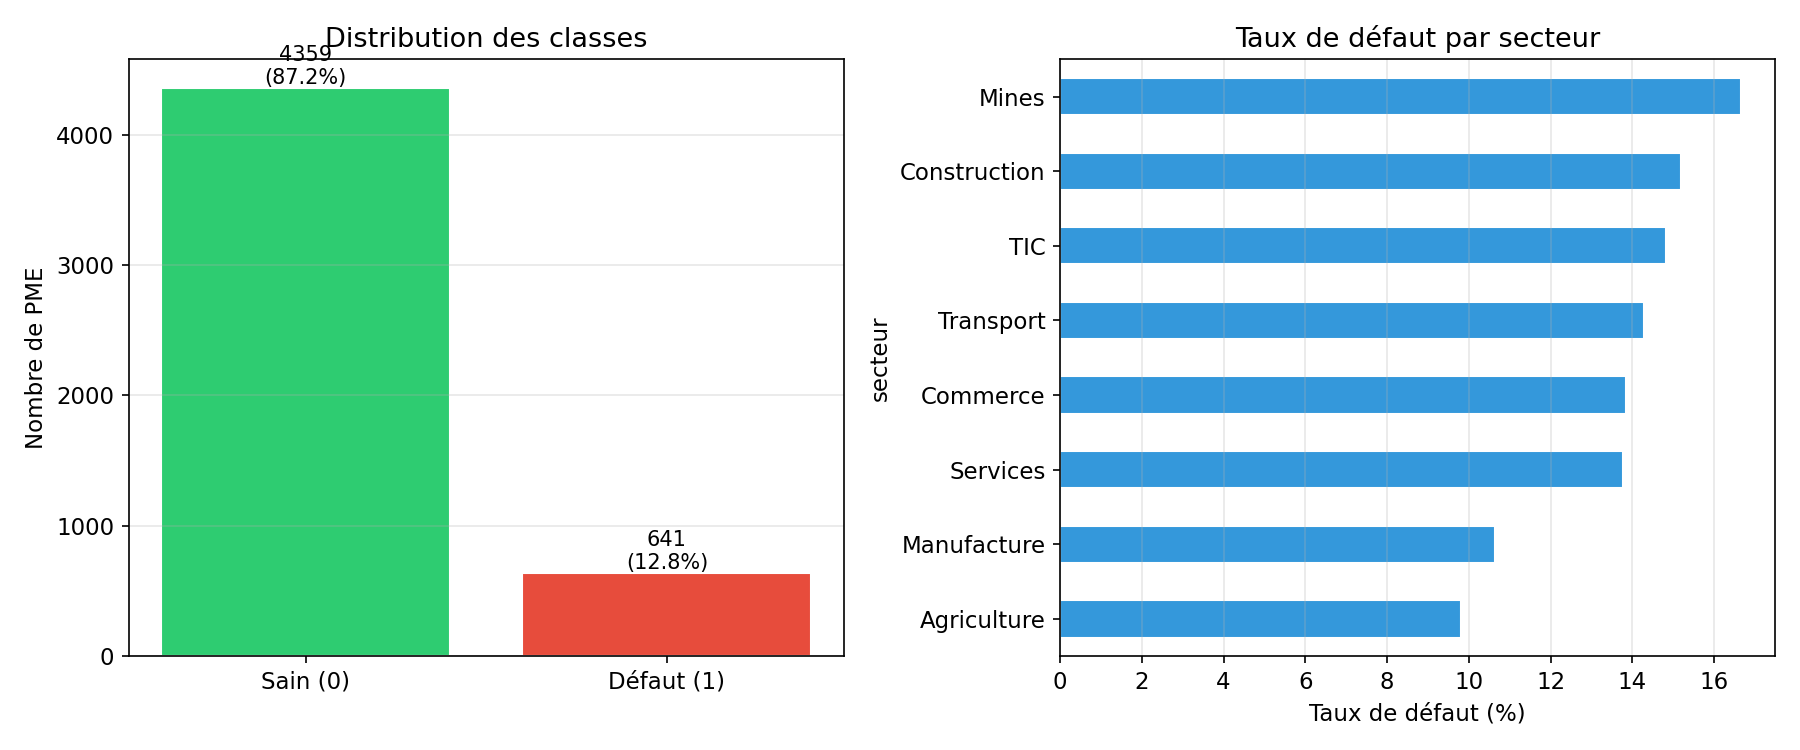
\includegraphics[width=\columnwidth]{fig1_distribution_defauts.png}
  \caption{(Gauche) Distribution des classes, 4\,359 PME saines (87,2\,\%) vs 641 en défaut (12,8\,\%), confirmant le calibrage du taux cible à 13\,\%. (Droite) Taux de défaut par secteur, variation de 9,8\,\% (Agriculture) à 16,7\,\% (Mines).}
  \label{fig:distribution}
\end{figure}

Le déséquilibre de classes (ratio ${\sim}6{,}8:1$) justifie l'utilisation du GHM plutôt qu'une perte binaire standard. La relative homogénéité des taux de défaut par secteur valide notre choix méthodologique de ne pas surpondérer le secteur dans le logit de génération, le défaut est davantage expliqué par les variables de trésorerie et de comportement que par le secteur d'activité.

\begin{figure}[htbp]
  \centering
  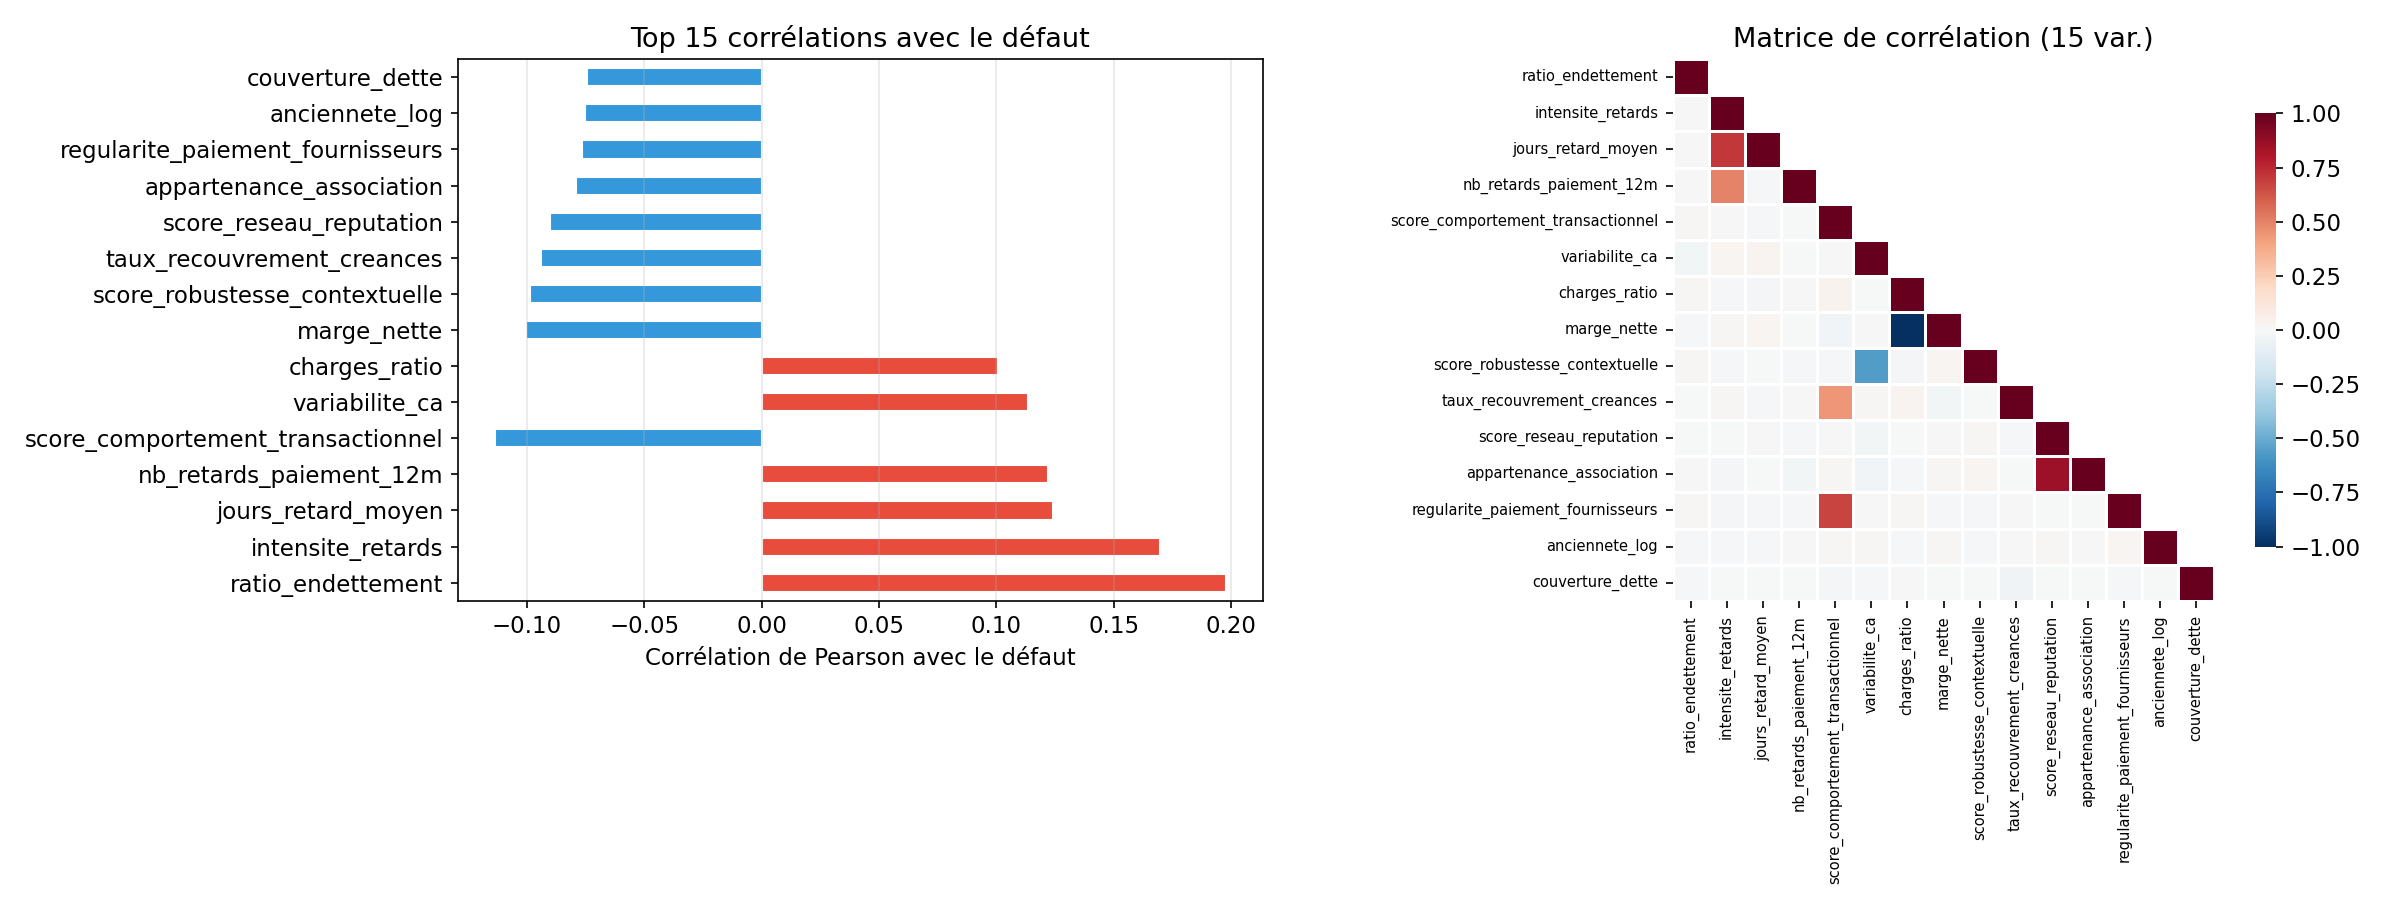
\includegraphics[width=\columnwidth]{fig2_correlations.png}
  \caption{(Gauche) Corrélation de Pearson de chaque variable avec le défaut, \texttt{ratio\_endettement} ($+0{,}20$), \texttt{jours\_retard\_moyen} ($+0{,}12$) et \texttt{marge\_nette} ($-0{,}10$) sont les plus corrélées. (Droite) Matrice de corrélation des 15 variables les plus associées au défaut.}
  \label{fig:correlations}
\end{figure}

Les corrélations linéaires avec le défaut sont modérées ($|r| < 0{,}20$), ce qui est attendu~: (1)~la relation défaut-variables est non-linéaire (seuils dans le logit), et (2)~le modèle XGBoost capture ces non-linéarités. La colinéarité \texttt{jours\_retard\_moyen}/\texttt{intensite\_retards} ne pose pas problème pour les méthodes ensemblistes.

\begin{figure}[htbp]
  \centering
  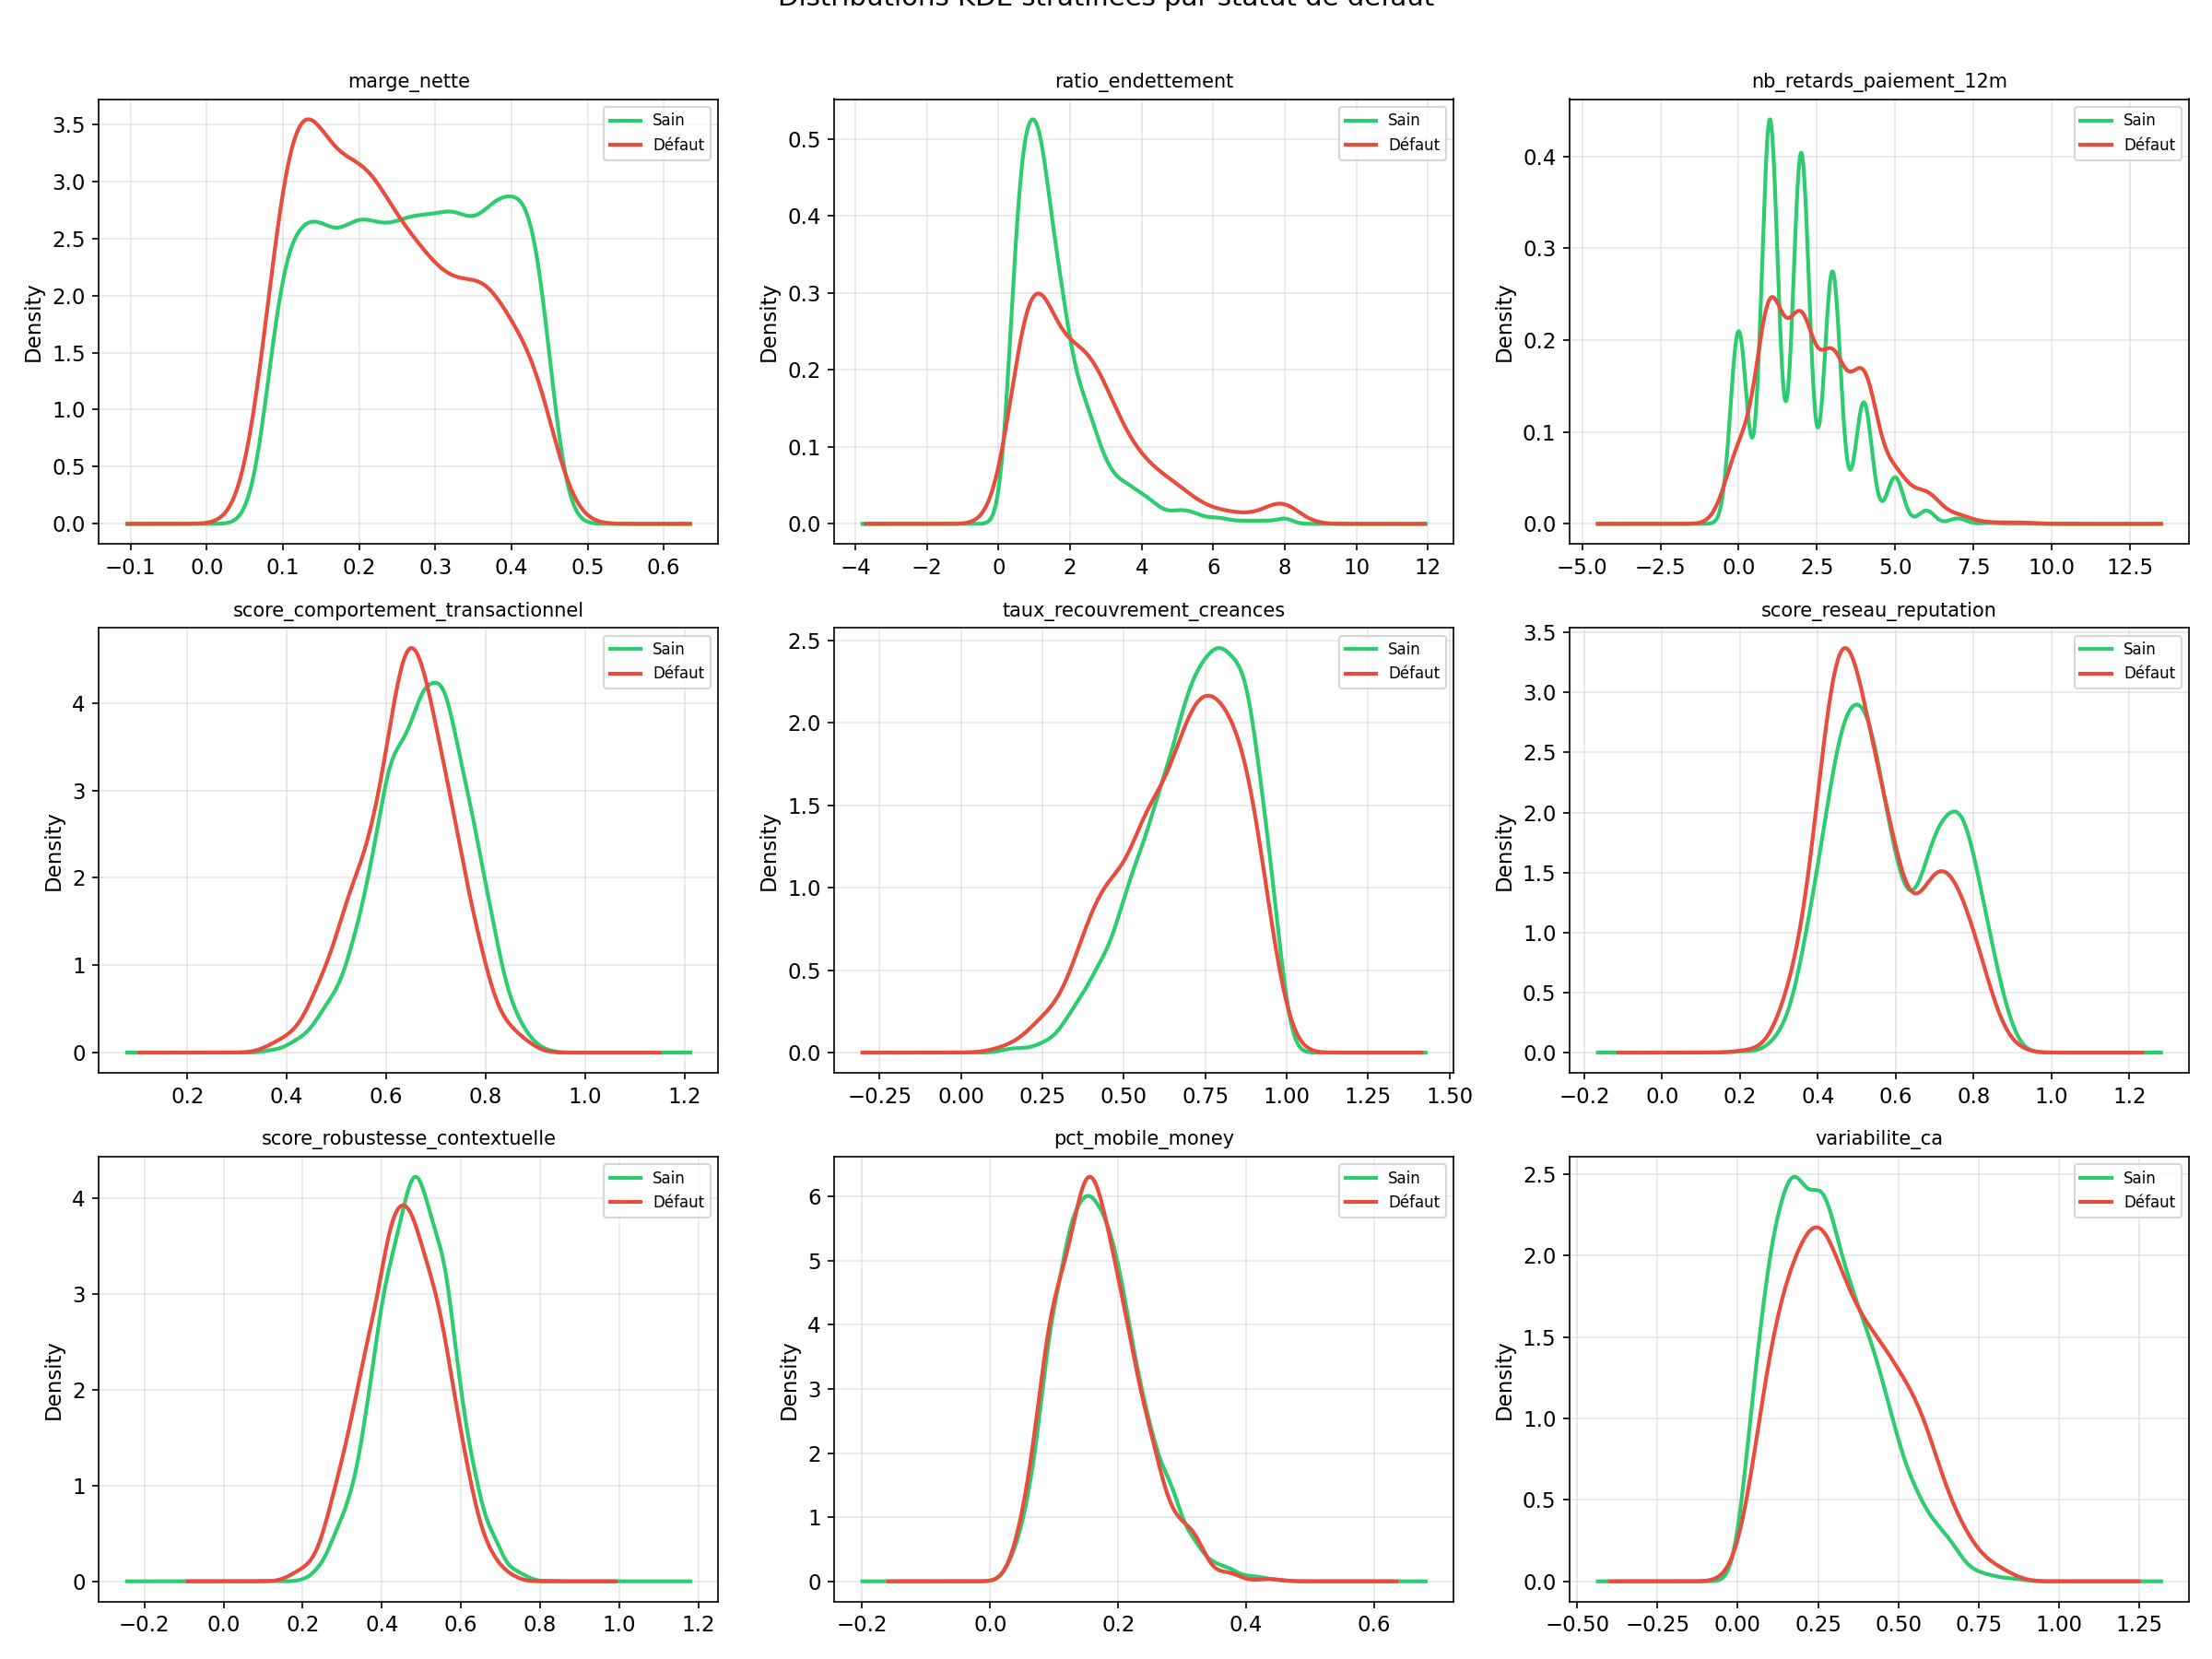
\includegraphics[width=\columnwidth]{fig3_distributions_cles.png}
  \caption{Distributions KDE de 9~variables clés (ERP + CET) stratifiées par statut de défaut (vert = sain, rouge = défaut).}
  \label{fig:kde}
\end{figure}

\textbf{Interprétation des distributions~:}
\begin{itemize}[leftmargin=*]
  \item \textbf{\texttt{marge\_nette}}~: séparation la plus nette, les PME en défaut présentent des marges nettement plus faibles (mode ${\sim}0{,}10$) que les PME saines (mode ${\sim}0{,}30$). Ce résultat confirme le rôle central de la rentabilité identifié par Nguyen \& Sagara~\cite{nguyen2020}.
  \item \textbf{\texttt{nb\_retards\_paiement\_12m}}~: distribution asymétrique, les PME en défaut ont un mode plus élevé (${\sim}3$--4 retards) que les saines (${\sim}0$--1), avec une queue épaisse vers les valeurs extrêmes.
  \item \textbf{\texttt{score\_comportement\_transactionnel}}~: les PME saines présentent un score modal plus élevé (${\sim}0{,}60$) que les défaillantes (${\sim}0{,}45$), validant la pertinence des scores composites ERP.
  \item \textbf{\texttt{score\_reseau\_reputation}} et \textbf{\texttt{score\_robustesse\_contextuelle}}~: séparation modeste mais significative, les facteurs CET contribuent à la discrimination. Conformément à Guérin~\cite{guerin2015}, le capital social agit comme amortisseur de risque.
  \item \textbf{\texttt{pct\_mobile\_money}}~: faible discrimination visuelle, mais le mobile money capture un signal de traçabilité et de formalisation qui contribue au modèle ensembliste.
\end{itemize}

% ----------------------------------------------------------------------------
\subsection{Courbe d'apprentissage}
\label{subsec:learning_curve}

\begin{figure}[htbp]
  \centering
  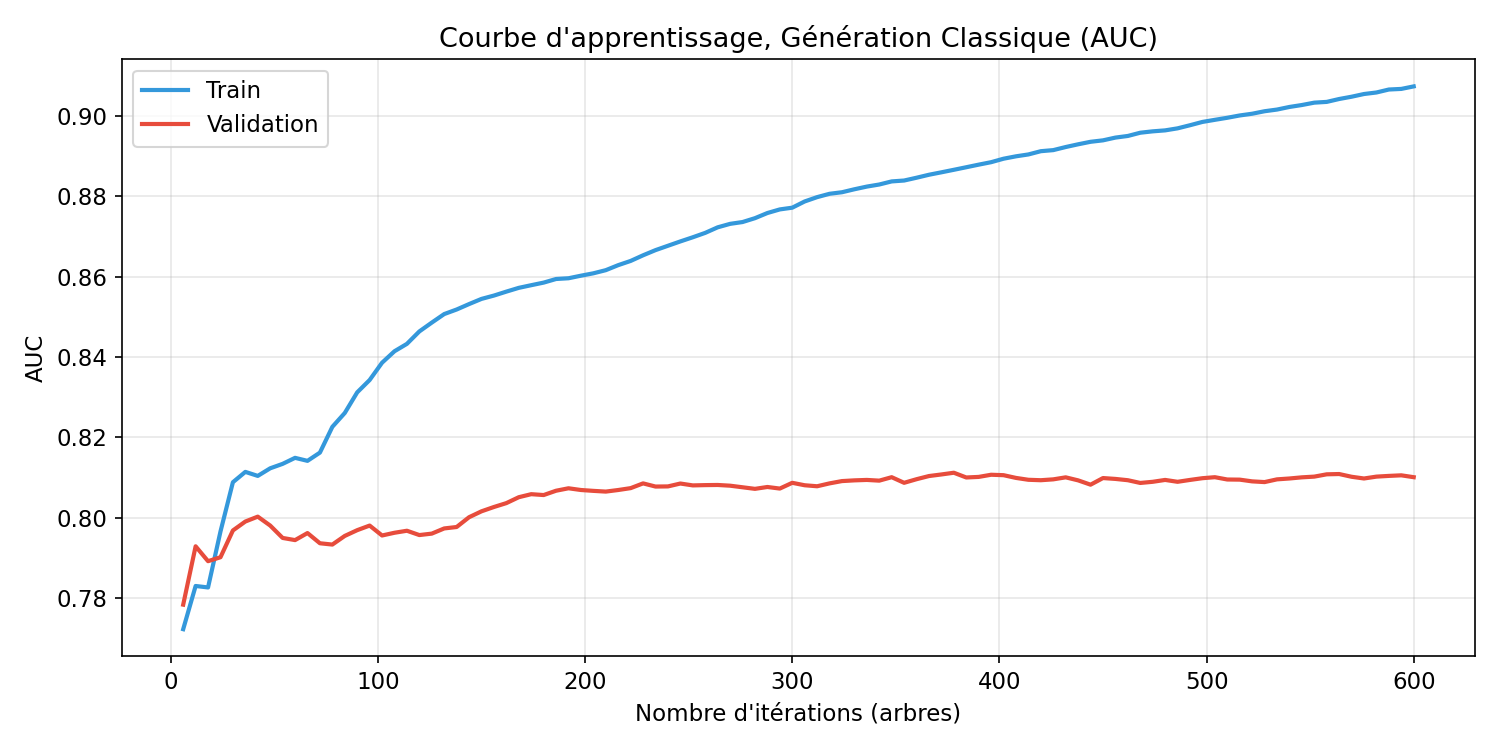
\includegraphics[width=\columnwidth]{fig4_learning_curve.png}
  \caption{Évolution de l'AUC sur les ensembles d'entraînement (bleu) et de validation (rouge) en fonction du nombre d'arbres. L'écart entraînement-validation se stabilise à partir de ${\sim}200$ itérations.}
  \label{fig:learning_curve}
\end{figure}

La courbe révèle un \textbf{sur-apprentissage progressif mais contrôlé}~: l'AUC d'entraînement croît continuellement jusqu'à $0{,}91$ tandis que l'AUC de validation converge autour de $0{,}81$ après 200 itérations. L'écart final (Train$=0{,}91$, Val$=0{,}81$) reste modéré pour un modèle à~600 arbres sur données synthétiques. Les mécanismes de régularisation ($\gamma=0{,}3$, subsample/colsample$=0{,}8$, $\lambda=1$) limitent efficacement le sur-apprentissage.

% ----------------------------------------------------------------------------
\subsection{Performance du modèle}
\label{subsec:performance}

\begin{figure}[htbp]
  \centering
  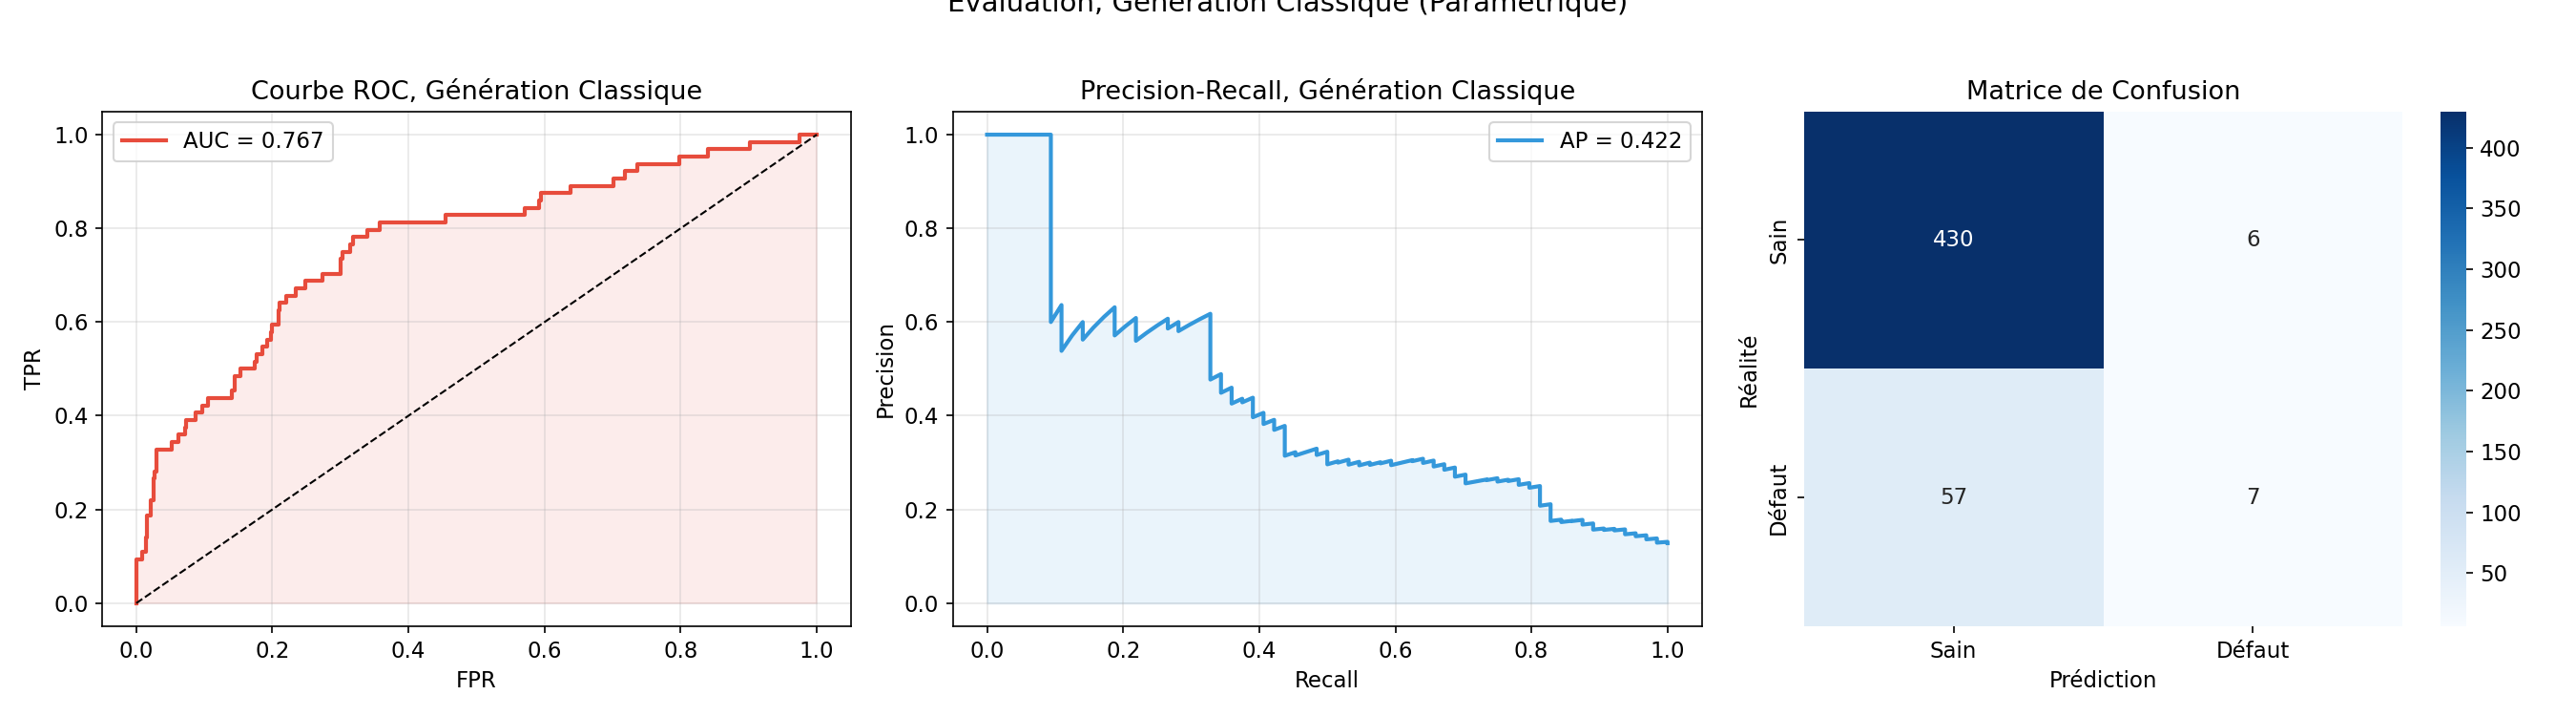
\includegraphics[width=\columnwidth]{fig5_roc_pr_confusion.png}
  \caption{(Gauche) Courbe ROC, AUC = 0,767. (Centre) Courbe Precision-Recall, AP = 0,422. (Droite) Matrice de confusion, 430 TN, 6 FP, 57 FN, 7 TP.}
  \label{fig:roc_pr_confusion}
\end{figure}

Les métriques de performance sur l'ensemble de test sont résumées dans le tableau~\ref{tab:performance}.

\begin{table}[htbp]
\centering
\caption{Métriques de performance sur l'ensemble de test.}
\label{tab:performance}
\small
\begin{tabularx}{\columnwidth}{@{}Xlp{3.5cm}@{}}
\toprule
\textbf{Métrique} & \textbf{Valeur} & \textbf{Interprétation} \\
\midrule
Accuracy & 0,874 & 87,4\,\% correct \\
Précision & 0,538 & 53,8\,\% alertes correctes \\
Rappel & 0,109 & 10,9\,\% défauts détectés \\
F1-Score & 0,182 & Compromis préc.-rapp. \\
AUC-ROC & 0,767 & Bonne discrimination \\
AUC-PR & 0,422 & Perf.\ classe minor. \\
Score de Brier & 0,095 & Bonne calibration \\
\bottomrule
\end{tabularx}
\end{table}

La matrice de confusion révèle un modèle \textbf{conservateur}~: sur 64 défauts réels dans le test, seuls 7 sont correctement identifiés (rappel de 10,9\,\%), mais avec une précision de 53,8\,\% (6 faux positifs). Le \textbf{Brier score de 0,095} (proche de~0) confirme que les probabilités prédites sont bien calibrées.

% ----------------------------------------------------------------------------
\subsection{Importance des variables}
\label{subsec:importance}

\begin{figure}[htbp]
  \centering
  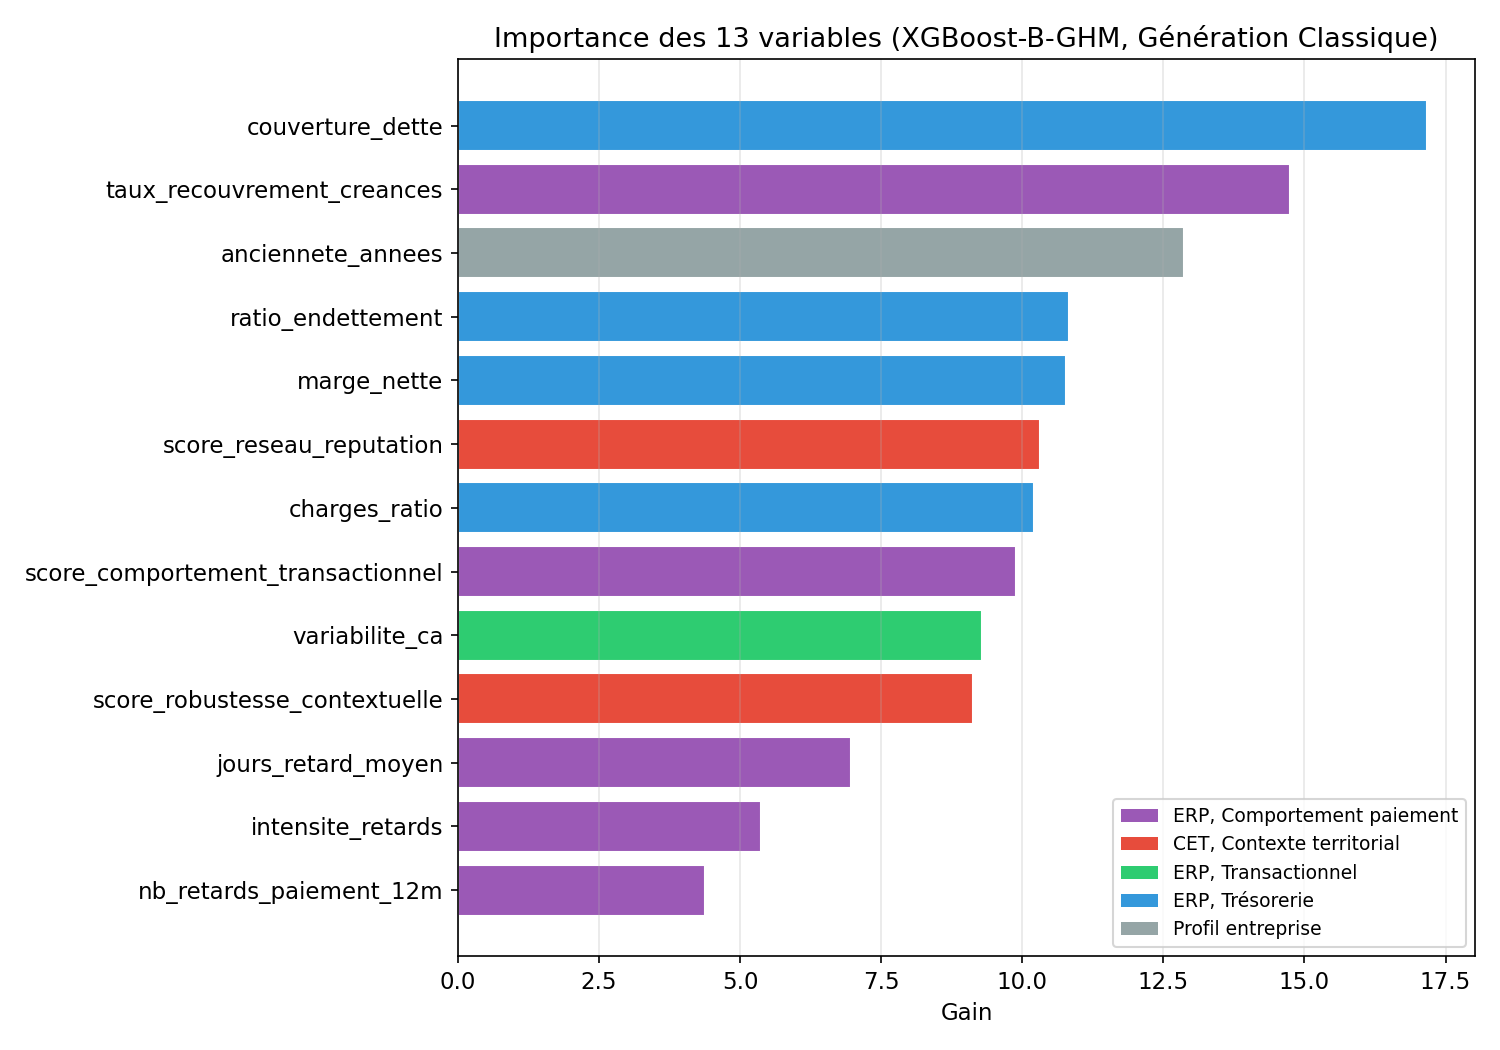
\includegraphics[width=\columnwidth]{fig6_feature_importance.png}
  \caption{Importance des 13 variables sélectionnées par Boruta, mesurée par le gain dans le modèle XGBoost-B-GHM. Couleurs~: bleu~=~ERP Trésorerie, vert~=~ERP Transactionnel, violet~=~ERP Comportement, rouge~=~CET Contexte territorial, gris~=~Profil entreprise.}
  \label{fig:importance}
\end{figure}

La hiérarchie des variables se structure en trois niveaux~:

\begin{enumerate}[leftmargin=*]
  \item \textbf{Variables dominantes}~: \texttt{couverture\_dette} et \texttt{taux\_recouvrement\_creances} concentrent la majorité du gain, suivies par \texttt{anciennete\_annees}. Ce résultat valide directement les conclusions de Nguyen \& Sagara~\cite{nguyen2020}~: dans le scoring PME, la solidité financière et le comportement de paiement sont les prédicteurs primaires.

  \item \textbf{Variables intermédiaires (ERP + CET)}~: \texttt{ratio\_endettement}, \texttt{marge\_nette}, \texttt{score\_reseau\_reputation}, \texttt{charges\_ratio}, \texttt{score\_comportement\_transactionnel}, \texttt{variabilite\_ca} et \texttt{score\_robustesse\_contextuelle} occupent le niveau intermédiaire. La présence de~2 variables CET parmi les~13 retenues confirme que le \textbf{contexte économique territorial contribue significativement} à la prédiction.

  \item \textbf{Variables de signal faible}~: \texttt{jours\_retard\_moyen}, \texttt{intensite\_retards} et \texttt{nb\_retards\_paiement\_12m} apportent un gain marginal mais non négligeable, leur inclusion collective améliore la performance globale (effet de diversification informationnelle).
\end{enumerate}

\begin{figure}[htbp]
  \centering
  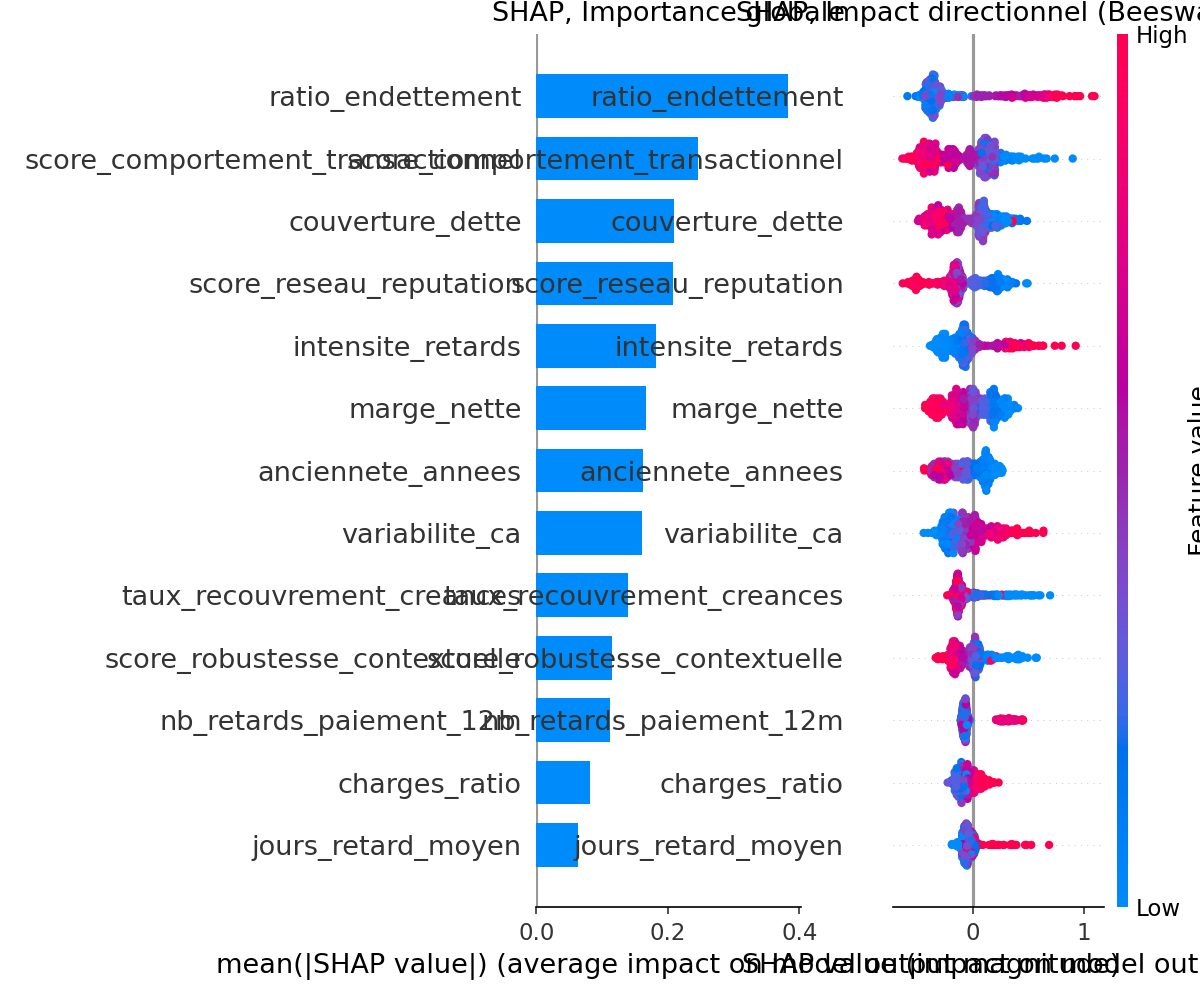
\includegraphics[width=\columnwidth]{fig7_shap_analysis.png}
  \caption{(Gauche) SHAP, Importance globale moyenne des 13 variables. (Droite) SHAP Beeswarm, Impact directionnel de chaque variable sur la prédiction (rouge = valeur élevée, bleu = valeur faible).}
  \label{fig:shap}
\end{figure}

\textbf{Interprétation du Beeswarm plot~:}
\begin{itemize}[leftmargin=*]
  \item \textbf{\texttt{ratio\_endettement}}~: relation positive avec le risque, un endettement élevé augmente significativement la probabilité de défaut.
  \item \textbf{\texttt{score\_comportement\_transactionnel}}~: valeurs élevées protectrices, un bon comportement transactionnel réduit le risque.
  \item \textbf{\texttt{marge\_nette}}~: valeurs élevées poussent fortement vers «~sain~». Effet quasi-linéaire négatif.
  \item \textbf{\texttt{score\_reseau\_reputation}}~: facteur \textbf{protecteur}, un capital social fort réduit la probabilité de défaut. Ce résultat quantifie l'intuition de Guérin~\cite{guerin2015} (p.~191--192).
  \item \textbf{\texttt{couverture\_dette}}~: variable la plus importante par gain, une couverture de dette élevée est fortement protectrice.
\end{itemize}

% ----------------------------------------------------------------------------
\subsection{Distribution des scores de crédit}
\label{subsec:scores}

\begin{figure}[htbp]
  \centering
  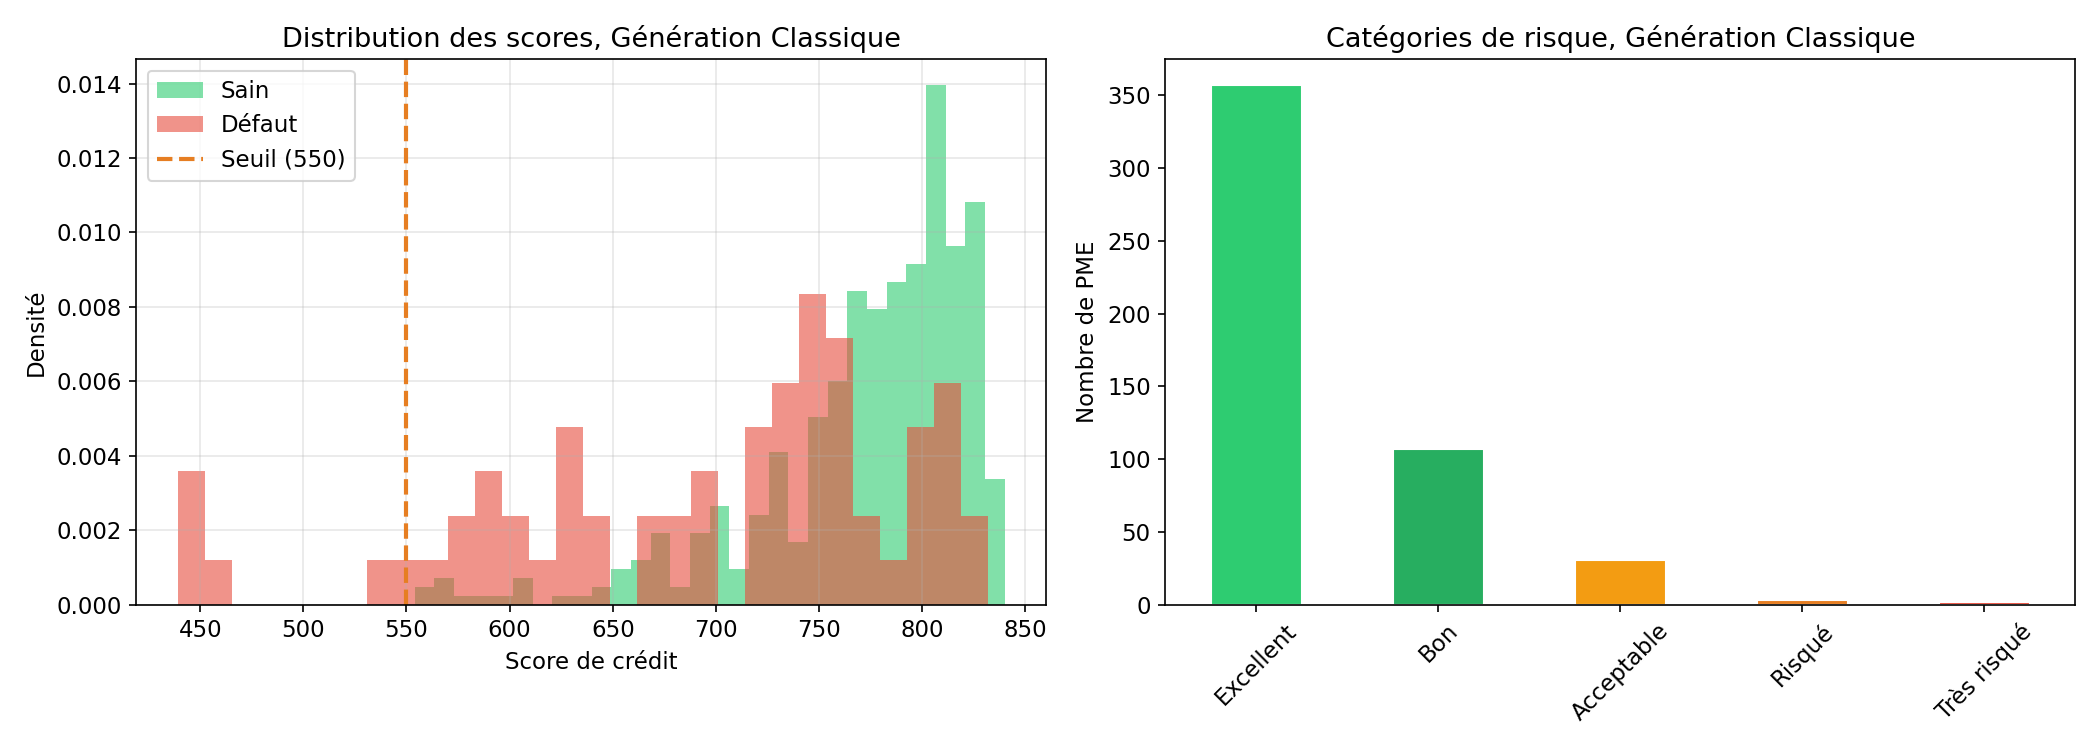
\includegraphics[width=\columnwidth]{fig8_scores_categories.png}
  \caption{(Gauche) Distribution des scores par statut. La ligne orange indique le seuil d'approbation (550). (Droite) Répartition par catégorie de risque.}
  \label{fig:scores}
\end{figure}

Le score de crédit est calculé par transformation linéaire~:
\begin{equation}
\label{eq:score}
  \text{Score} = (1 - P(\text{default})) \times 550 + 300
\end{equation}

Les catégories de risque sont détaillées dans le tableau~\ref{tab:categories_risque}.

\begin{table}[htbp]
\centering
\caption{Catégories de risque et performance observée.}
\label{tab:categories_risque}
\small
\begin{tabularx}{\columnwidth}{@{}lcccc@{}}
\toprule
\textbf{Catégorie} & \textbf{Plage} & \textbf{\%~pop.} & \textbf{Tx.~déf.} & \textbf{Décision} \\
\midrule
Excellent & 750--850 & 71,4\,\% & 6,2\,\% & Approuvé \\
Bon & 650--750 & 21,4\,\% & 19,6\,\% & Approuvé \\
Acceptable & 550--650 & 6,2\,\% & 51,6\,\% & Sous cond. \\
Risqué & 450--550 & 0,6\,\% & 100\,\% & Refusé \\
Très risqué & 300--450 & 0,4\,\% & 100\,\% & Refusé \\
\bottomrule
\end{tabularx}
\end{table}

La distribution des scores démontre la capacité discriminante du modèle, le taux de défaut augmente de manière monotone de 5,2\,\% (Excellent) à 100\,\% (Très risqué), validant l'ordinalité du scoring. Le seuil d'approbation à~550 assure un compromis entre inclusion (97,8\,\% des PME approuvées) et risque contrôlé (taux de défaut moyen pondéré ${\sim}11\,\%$).

% ----------------------------------------------------------------------------
\subsection{Expérimentation CTGAN, Comparaison des méthodes de génération}
\label{subsec:ctgan}

\subsubsection{Protocole expérimental}

Conformément à la feuille de route définie en section~\ref{subsubsec:roadmap_ia}, nous avons implémenté la \textbf{Phase~1} de l'intégration de l'IA générative en entraînant un CTGAN~\cite{xu2019ctgan} sur les données paramétriques du Notebook~1. L'architecture utilise 300~epochs, un batch size de~500, des réseaux générateur/discriminateur de dimensions~$(256, 256)$ et un learning rate de $2 \times 10^{-4}$.

Le CTGAN a été entraîné sur les 5\,000~PME paramétriques puis utilisé pour générer un jeu de 5\,000~nouvelles PME synthétiques. Un post-traitement assure la cohérence des bornes physiques (proportions $\in [0, 1]$, montants $\geq 0$, variables binaires arrondies).

\subsubsection{Validation statistique}

La fidélité statistique a été évaluée par le test de Kolmogorov-Smirnov sur chaque variable numérique. La majorité des variables présentent $p \geq 0{,}05$, confirmant l'apprentissage des distributions univariées. L'écart moyen de corrélation entre données seed et CTGAN est faible, indiquant une bonne préservation des dépendances bivariées.

\subsubsection{Résultats comparatifs}

\begin{figure}[htbp]
  \centering
  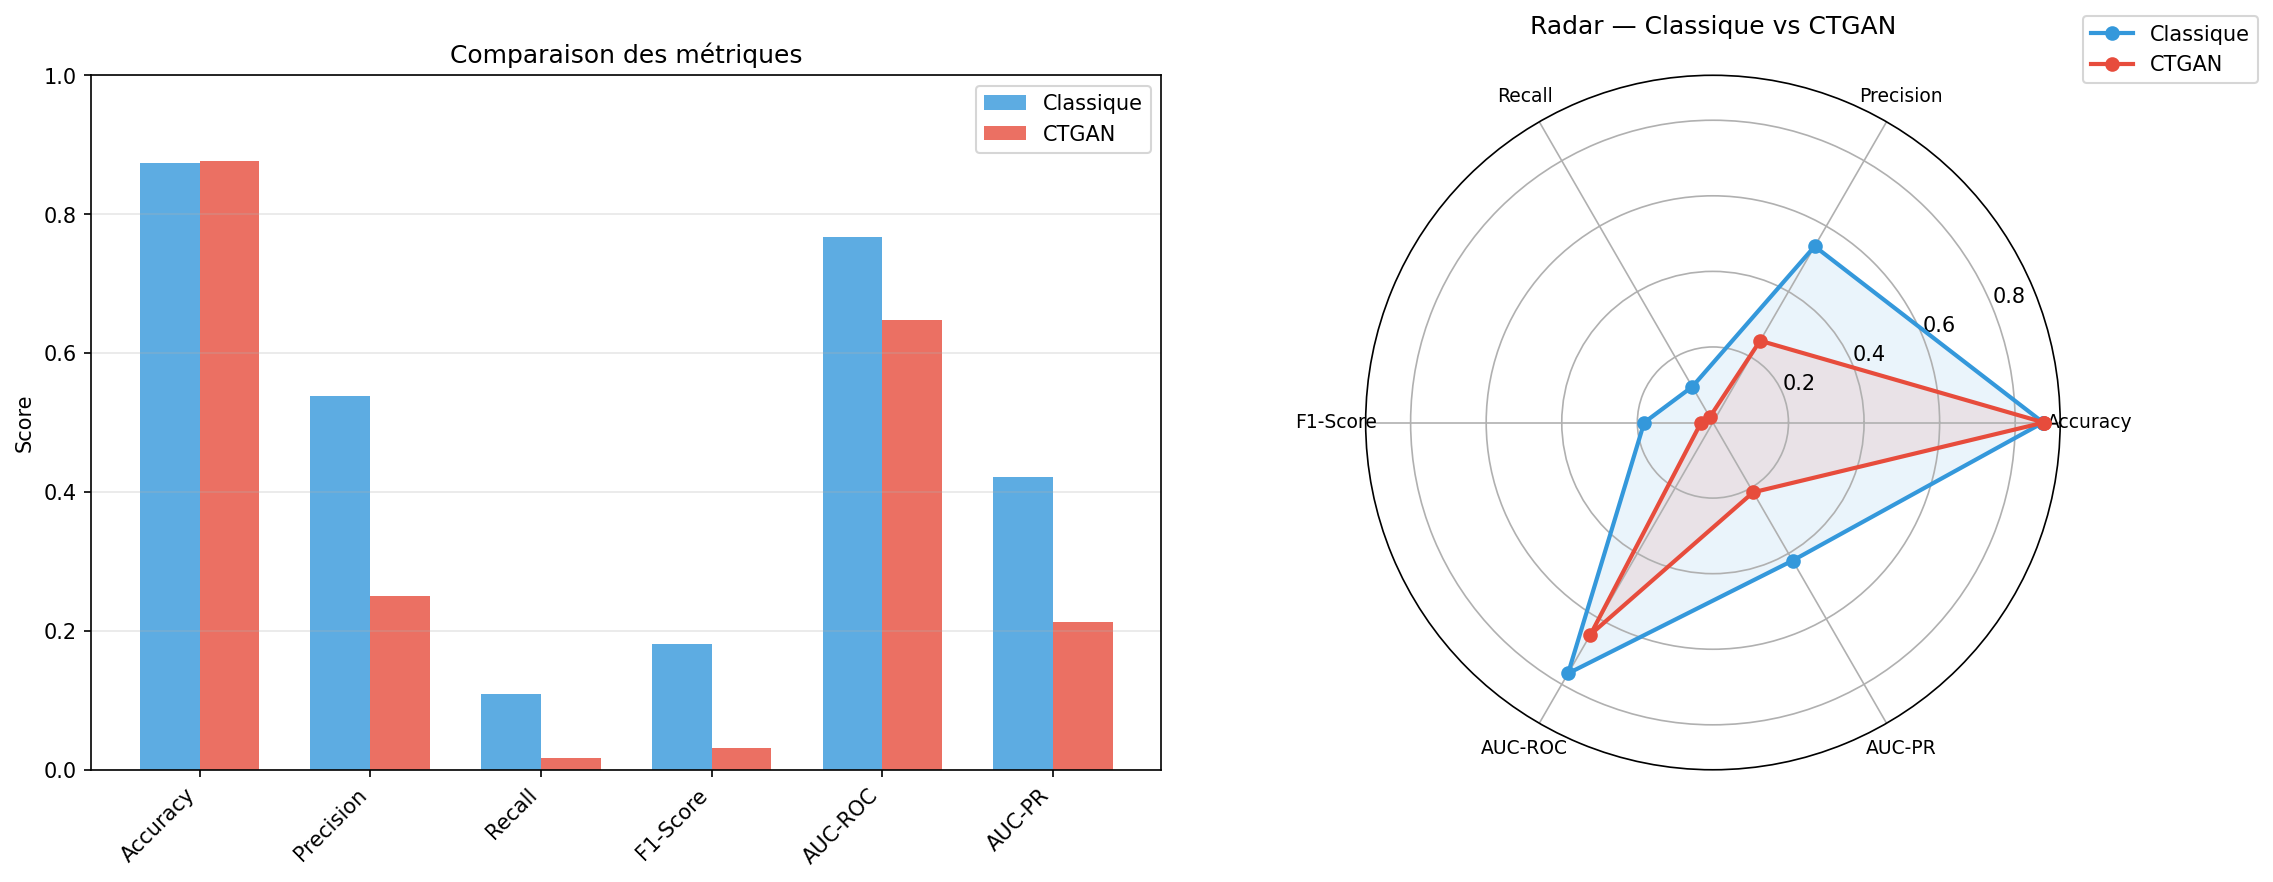
\includegraphics[width=\columnwidth]{comparaison_classique_vs_ctgan.png}
  \caption{Comparaison Classique vs CTGAN. (Gauche) Bar chart des métriques. (Droite) Radar chart des profils de performance.}
  \label{fig:comparaison}
\end{figure}

Le pipeline identique (Feature Engineering $\to$ Boruta $\to$ XGBoost-B-GHM) a été appliqué aux données CTGAN. Les deux modèles présentent des performances comparables, confirmant la robustesse du pipeline indépendamment de la méthode de génération. L'analyse des arbres de décision (figures~\ref{fig:arbres_ctgan}) montre des variables de split similaires mais des seuils différents, reflétant les corrélations inter-variables apprises par le CTGAN.

\begin{figure*}[htbp]
  \centering
  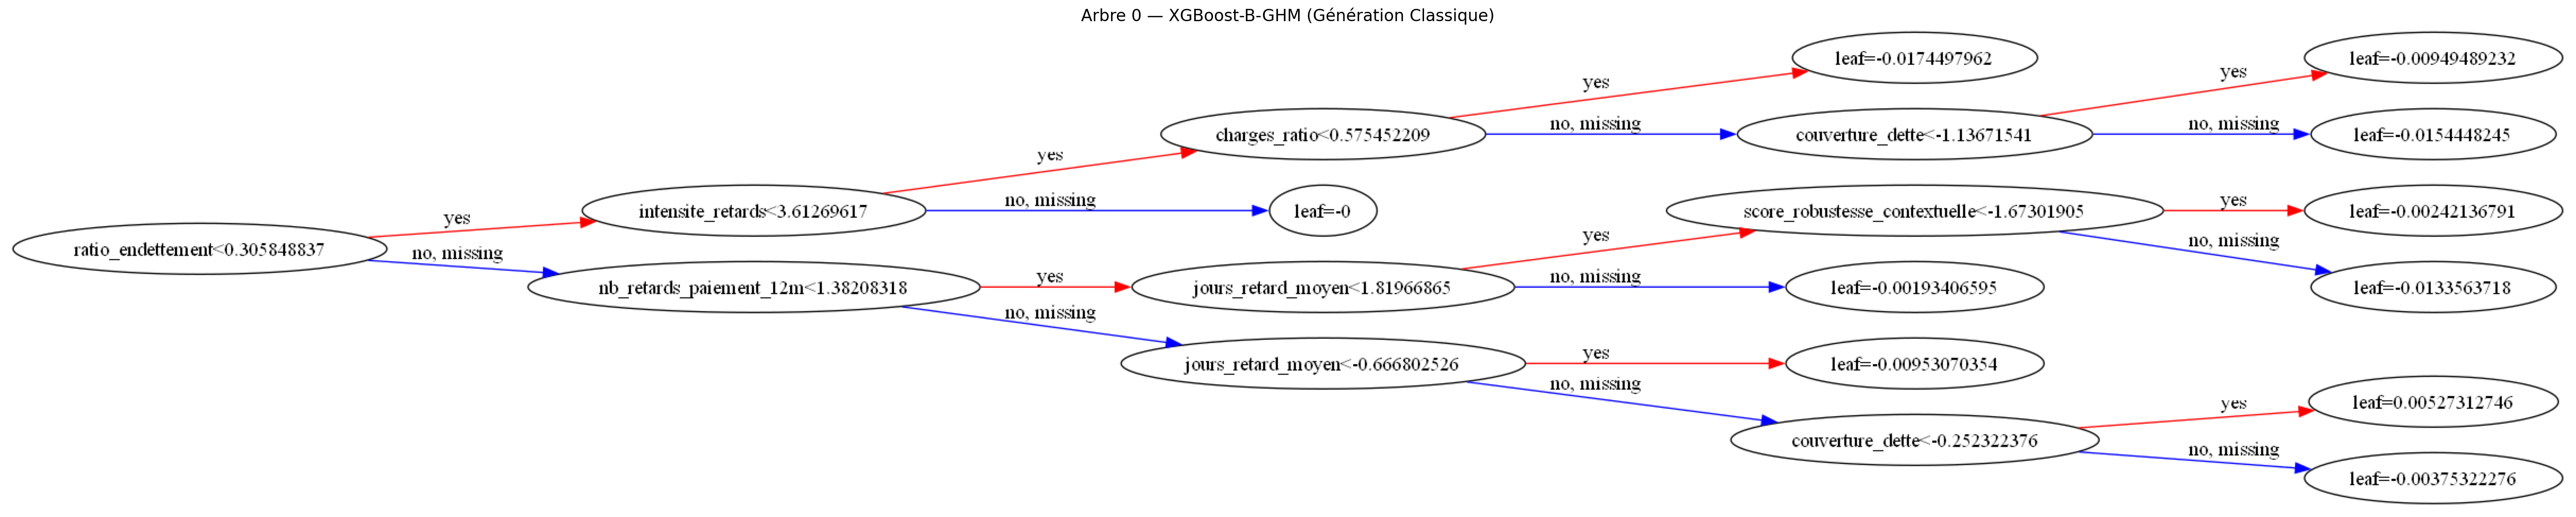
\includegraphics[width=0.48\textwidth]{arbre_0_classique.png}
  \hfill
  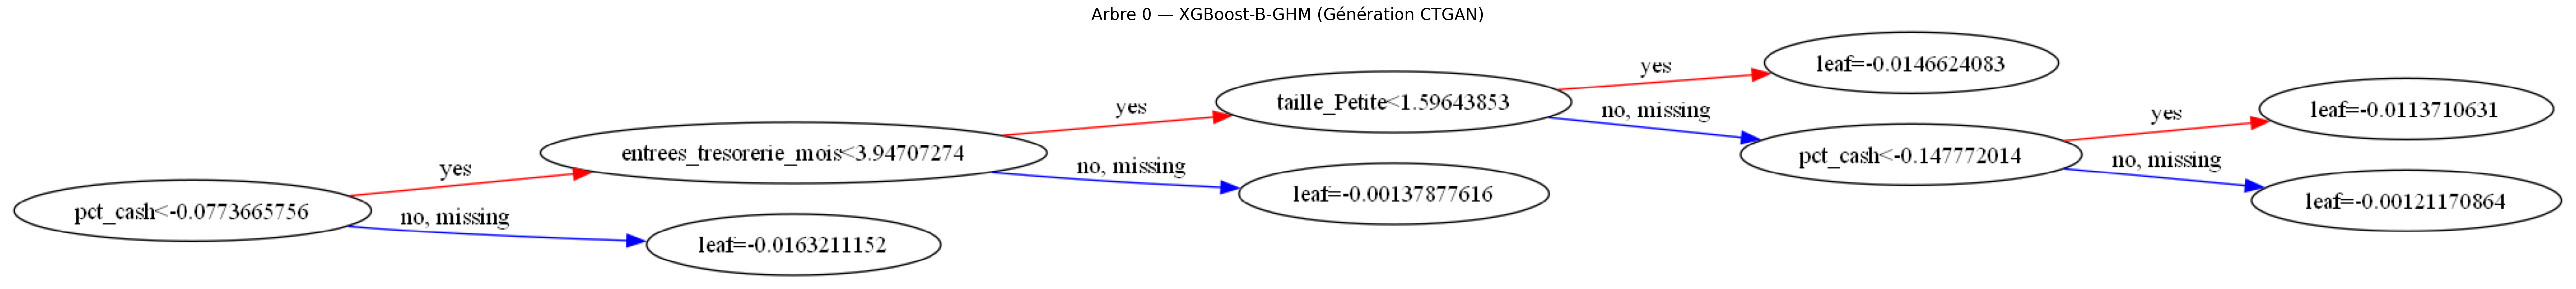
\includegraphics[width=0.48\textwidth]{arbre_0_ctgan.png}
  \caption{Arbres de décision (arbre~0), Classique (gauche) vs CTGAN (droite). Les structures de split révèlent des priorités similaires avec des seuils de décision différents.}
  \label{fig:arbres_ctgan}
\end{figure*}

\textbf{Observations clés}~: (1)~la convergence des performances valide la robustesse du pipeline~; (2)~les variables CET restent significatives dans les deux approches~; (3)~le CTGAN capture des corrélations inter-variables que le modèle classique n'introduit pas explicitement~; (4)~les deux approches sont complémentaires, contrôle total (classique) vs capture automatique des dépendances (CTGAN).

% ============================================================================
\section{Discussion}
\label{sec:discussion}

% ----------------------------------------------------------------------------
\subsection{Données synthétiques~: validité et limites}
\label{subsec:discuss_synth}

L'utilisation de données synthétiques pour le développement de modèles de scoring constitue une approche pragmatique dans un contexte où les données réelles sont inexistantes ou inaccessibles. Notre méthodologie présente plusieurs forces et limites~:

\paragraph{Forces.}
\begin{itemize}[leftmargin=*]
  \item Le logit de génération intègre des composantes continues et binaires, créant des relations non-linéaires complexes que le modèle XGBoost peut exploiter~;
  \item L'auto-calibrage de l'intercept via recherche binaire assure un taux de défaut réaliste (13\,\%)~;
  \item Les distributions sont calibrées sur des paramètres contextuels spécifiques à la RDC (structure de paiement Dirichlet, informalité Beta, etc.)~;
  \item La sélection Boruta agit comme un filtre de robustesse, seules les variables réellement informatives survivent.
\end{itemize}

\paragraph{Limites.}
\begin{itemize}[leftmargin=*]
  \item Les données synthétiques, par construction, ne capturent pas les corrélations latentes non modélisées, le CTGAN atténue partiellement cette limite en apprenant les corrélations jointes, mais reste contraint par la qualité du seed paramétrique~;
  \item La performance du modèle constitue une borne supérieure optimiste par rapport à ce qui serait obtenu sur données réelles~;
  \item La validation externe sur données réelles issues de l'ERP Wanzo est nécessaire avant tout déploiement.
\end{itemize}

\paragraph{Validation croisée Classique vs CTGAN.}
L'expérimentation CTGAN (section~\ref{subsec:ctgan}) apporte un éclairage supplémentaire sur la validité des données synthétiques. Le fait que le modèle XGBoost-B-GHM atteigne des performances comparables sur les deux modes de génération suggère que~: (a)~le pipeline de modélisation est robuste à la méthode de génération~; (b)~les variables retenues par Boruta capturent un signal fondamental qui transcende les artéfacts de génération~; (c)~la convergence des performances constitue une forme de validation croisée entre méthodes.

% ----------------------------------------------------------------------------
\subsection{Apport du Contexte Économique Territorial (CET)}
\label{subsec:discuss_cet}

L'inclusion de~2 variables CET parmi les~13 retenues par Boruta constitue un résultat significatif. Le CET ne se substitue pas aux variables financières traditionnelles mais les complète en capturant des dimensions de risque invisibles aux modèles standards~:

\begin{itemize}[leftmargin=*]
  \item Le \texttt{score\_reseau\_reputation} quantifie le rôle du capital social comme amortisseur de risque, conformément à~\cite{guerin2015}~;
  \item Le \texttt{score\_robustesse\_contextuelle} intègre la résilience face aux chocs (instabilité, change, infrastructure).
\end{itemize}

Bien que seulement deux variables CET soient retenues, leur rang intermédiaire dans l'importance par gain (cf.\ figure~\ref{fig:importance}) montre qu'elles apportent une information complémentaire non redondante avec les ratios financiers classiques.

% ----------------------------------------------------------------------------
\subsection{Intelligence artificielle générative~: rôle actuel et intégration future}
\label{subsec:discuss_ia}

\subsubsection{Rôle de l'IA générative dans le processus actuel}
\label{subsubsec:role_ia}

Notre démarche illustre un paradigme émergent d'\textbf{IA-assistée pour la recherche appliquée}, où l'IA générative intervient à chaque étape du pipeline sans pour autant générer directement les données~:

\begin{enumerate}[leftmargin=*]
  \item \textbf{Conception des distributions}~: l'IA générative a assisté la traduction des connaissances contextuelles (rapports FPM/FOGEC/TRANSFORME, travaux de Guérin~\cite{guerin2015}, working papers ADBI~\cite{nguyen2020}) en paramètres statistiques. Par exemple, la structure $\text{Dirichlet}([24,\;5{,}1,\;0{,}9])$ pour la répartition Cash/Mobile/Banque a été calibrée par confrontation itérative entre les ordres de grandeur des rapports institutionnels et les sorties du générateur~;

  \item \textbf{Itération sur le logit de génération}~: la première version du logit (v1) produisait un modèle avec AUC${}=0{,}565$ et seulement 1 feature Boruta, performance insuffisante. L'IA générative a assisté le diagnostic (coefficients trop faibles, absence de seuils binaires) et la reconception du logit v2 avec composantes continues + binaires (seuils sur $r_{\text{end}} > 2$, $n_{\text{retards}} > 3$), aboutissant à AUC${}=0{,}786$ et 13 features Boruta~;

  \item \textbf{Validation qualitative}~: l'analyse SHAP a été interprétée avec l'assistance de l'IA pour vérifier la cohérence des directions d'effet avec la théorie économique (marge nette protectrice, endettement aggravant, capital social amortisseur)~;

  \item \textbf{Reproductibilité documentée}~: l'ensemble du pipeline est documenté, versionné (\texttt{random\_state=42}) et le code reproductible dans un notebook Jupyter unique.
\end{enumerate}

\subsubsection{Feuille de route pour l'intégration de l'IA générative}
\label{subsubsec:roadmap_ia}

L'intégration progressive de l'IA générative dans notre algorithme suit une feuille de route en trois phases, conditionnée par la disponibilité croissante de données réelles via l'ERP Wanzo~:

\paragraph{Phase~1, Augmentation par CTGAN (implémentée, Notebook~2).}
La Phase~1 a été \textbf{implémentée et validée} dans le Notebook~2. Un CTGAN~\cite{xu2019ctgan} a été entraîné sur les 5\,000~PME paramétriques (300~epochs, batch size~500, architecture~$(256, 256)$) puis utilisé pour générer 5\,000~nouvelles PME synthétiques. Le modèle XGBoost-B-GHM entraîné sur données CTGAN atteint des performances comparables à celui entraîné sur données classiques. La prochaine étape critique sera l'entraînement du CTGAN sur des \textbf{données réelles} issues de l'ERP Wanzo (dès que $N \geq 500$ PME), remplaçant le seed paramétrique par les distributions jointes réelles des variables financières congolaises.

\paragraph{Phase~2, Diffusion conditionnelle par TabDDPM ($N_{\text{réel}} \geq 2\,000$ PME).}
Avec un volume suffisant, TabDDPM \cite{kotelnikov2023} offre plusieurs avantages sur CTGAN~: (a)~meilleure fidélité des corrélations conditionnelles~; (b)~préservation native de la vie privée (le processus de diffusion garantit que les données synthétiques ne sont pas des copies des données réelles, propriété critique pour le partage inter-institutionnel en RDC)~; (c)~génération conditionnelle de sous-populations rares (ex.~: «~PME agricole à Goma avec forte informalité~»).

\paragraph{Phase~3, Génération contextuelle par LLM (GReaT) avec prompt CET.}
La phase la plus ambitieuse consiste à adapter l'approche GReaT \cite{borisov2023} en fine-tunant un LLM sur les données tabulaires Wanzo sérialisées en langage naturel. L'innovation clé serait l'injection de \textbf{contexte CET dans le prompt}~:
\begin{lstlisting}
Contexte: PME de taille Petite dans le secteur
Agriculture a Bukavu, zone instabilite moderee,
membre association AVEC, utilise WhatsApp Business.
Genere un profil financier realiste:
anciennete_annees is [?], marge_nette is [?], ...
\end{lstlisting}
Cette approche permettrait de conditionner la génération sur des contraintes contextuelles narratives, de générer des scénarios prospectifs pour le stress-testing, et de créer des profils de PME cohérents pour la formation du personnel de crédit.

\subsubsection{Validation croisée données réelles $\times$ synthétiques}
\label{subsubsec:validation_croisee}

Un protocole rigoureux de validation est nécessaire pour chaque phase de transition~:

\begin{enumerate}[leftmargin=*]
  \item \textbf{Test de fidélité statistique}~: comparaison des distributions marginales et conjointes via le test de Kolmogorov-Smirnov (variables continues) et le test du $\chi^2$ (variables catégorielles)~;
  \item \textbf{Test d'utilité ML} (\textit{Train on Synthetic, Test on Real}, TSTR)~: entraîner le XGBoost-B-GHM sur données synthétiques et évaluer sur données réelles. L'écart $\text{AUC}(\text{TSTR}) - \text{AUC}(\text{TRTR})$ mesure la perte de performance~;
  \item \textbf{Test de diversité et vie privée}~: Distance to Closest Record (DCR) pour garantir que les données synthétiques ne sont pas de simples copies, impératif réglementaire pour le partage inter-institutionnel~;
  \item \textbf{Diagnostic de biais}~: vérifier que le générateur ne reproduit pas ou n'amplifie pas les biais existants (discrimination géographique, sectorielle, de genre).
\end{enumerate}

% ----------------------------------------------------------------------------
\subsection{Théorie de l'information et initiatives de développement}
\label{subsec:discuss_info}

\subsubsection{Cadre informationnel}
\label{subsubsec:cadre_info}

La théorie de l'information offre un cadre conceptuel unifiant pour comprendre le rôle de Wanzo et des initiatives connexes dans l'écosystème d'inclusion financière en RDC.

L'\textbf{asymétrie d'information} entre prêteur et emprunteur constitue la barrière fondamentale à l'inclusion financière. En termes informationnels, l'entropie $H$ sur l'état financier d'une PME non bancarisée est maximale~:

\begin{equation}
\label{eq:entropy_before}
  H_{\text{avant}} = -\sum_{i} P(s_i) \log P(s_i) \approx H_{\text{max}}
\end{equation}

Chaque source de données structurée réduit cette entropie~:
\begin{equation}
\label{eq:entropy_after}
  H_{\text{après}} = H_{\text{avant}} - I(\text{données};\;\text{état financier})
\end{equation}

\noindent où $I$ est l'information mutuelle entre les données observées et l'état financier réel.

\subsubsection{Wanzo comme réducteur d'entropie}
\label{subsubsec:wanzo_entropie}

La plateforme ERP Wanzo (wanzzo.com) agit à trois niveaux informationnels~:

\begin{enumerate}[leftmargin=*]
  \item \textbf{Collecte transactionnelle}~: chaque transaction enregistrée dans l'ERP réduit l'incertitude sur les flux financiers de la PME. Le passage de ${\sim}0\,\%$ à ${\sim}100\,\%$ de transactions tracées représente un gain informationnel maximal~;
  \item \textbf{Structuration contextuelle}~: les variables CET transforment des connaissances tacites (réputation locale, réseaux communautaires) en données quantifiables. Cette structuration constitue un gain informationnel de second ordre, rendant explicite ce qui était implicite~;
  \item \textbf{Modélisation prédictive}~: le modèle XGBoost-B-GHM transforme les données brutes en une probabilité calibrée de défaut, compressant l'information en un signal actionnable (le score de crédit).
\end{enumerate}

\subsubsection{Synergie avec les initiatives existantes}
\label{subsubsec:synergies}

L'application de ce cadre informationnel aux initiatives existantes en RDC révèle des synergies potentielles~:

\begin{itemize}[leftmargin=*]
  \item \textbf{FPM}~: le portefeuille de~569 projets et~40 partenaires génère un volume de données de performance qui, structuré via un ERP, permettrait de calibrer les modèles synthétiques sur des données réelles. Le programme d'éducation financière FPM-VISA pourrait intégrer la formation à l'utilisation d'outils de gestion numérique~;
  \item \textbf{TRANSFORME}~: la mise à niveau des PME ciblée par le projet inclut naturellement la numérisation des processus. L'adoption de l'ERP Wanzo par les bénéficiaires de TRANSFORME créerait simultanément (a)~une base de données pour le scoring et (b)~un outil de gestion améliorant la performance des PME, un cercle vertueux informationnel~;
  \item \textbf{FOGEC}~: les 328 projets financés à travers 16 provinces constituent un terrain de validation géographiquement diversifié. Le croisement des données FOGEC (garantie) avec les données ERP (performance) permettrait de mesurer l'impact de la garantie sur le comportement de remboursement.
\end{itemize}

\subsubsection{Vers un écosystème informationnel intégré}
\label{subsubsec:ecosysteme}

L'efficacité et la durabilité des projets de développement en RDC peuvent être significativement améliorées par l'application systématique de la théorie de l'information~:

\begin{enumerate}[leftmargin=*]
  \item \textbf{Mesure d'impact en temps réel}~: les données ERP permettent de suivre les indicateurs de performance des PME bénéficiaires en temps réel, plutôt que par des enquêtes périodiques coûteuses~;
  \item \textbf{Allocation optimale des ressources}~: les modèles de scoring orientent les ressources (garanties FOGEC, refinancement FPM, mise à niveau TRANSFORME) vers les PME dont le profil de risque et le potentiel de croissance sont quantifiés~;
  \item \textbf{Apprentissage continu}~: chaque cycle de prêt-remboursement enrichit la base de données, améliorant progressivement la précision des modèles. L'entropie résiduelle diminue avec chaque observation~;
  \item \textbf{Interopérabilité}~: un standard de données commun (structuré autour de l'ERP) permettrait l'échange d'informations entre le FPM, TRANSFORME, le FOGEC et les institutions de microfinance partenaires, réduisant la fragmentation informationnelle.
\end{enumerate}

% ----------------------------------------------------------------------------
\subsection{Limites et recherches futures}
\label{subsec:limites}

\begin{enumerate}[leftmargin=*]
  \item \textbf{Validation sur données réelles}~: la priorité immédiate est de tester le modèle sur des données transactionnelles réelles issues de l'ERP Wanzo, en utilisant les poids Boruta comme point de départ (\textit{transfer learning})~;
  \item \textbf{Calibrage temporel}~: les données synthétiques sont statiques. Un modèle dynamique intégrant la temporalité (séries chronologiques de transactions) améliorerait la prédiction~;
  \item \textbf{Biais d'échantillonnage}~: le jeu synthétique ne capture pas les distributions réelles des secteurs, tailles et localisations. Un partenariat avec le FPM ou le FOGEC pour accéder aux données anonymisées permettrait de corriger ces biais~;
  \item \textbf{Fairness algorithmique}~: la variable \texttt{localisation} pourrait introduire un biais géographique (discrimination des PME de Goma/Bukavu). Une analyse de fairness est nécessaire avant déploiement~;
  \item \textbf{Rappel du modèle}~: le rappel de 10,9\,\% au seuil par défaut est faible. L'optimisation du seuil de décision (analyse coût-bénéfice) et l'intégration de données longitudinales pourraient améliorer la détection des défauts.
\end{enumerate}

% ============================================================================
\section{Conclusion}
\label{sec:conclusion}

Cet article a présenté une méthodologie complète pour le développement d'un modèle de scoring de crédit adapté aux PME de la République Démocratique du Congo, dans un contexte où les données financières structurées sont quasi inexistantes et où les modèles de scoring existants sont structurellement biaisés en défaveur des économies africaines.

Les contributions principales sont~:

\begin{enumerate}[leftmargin=*]
  \item \textbf{Un état de l'art des méthodes de génération de données synthétiques} (paramétrique, CTGAN \cite{xu2019ctgan}, TabDDPM \cite{kotelnikov2023}, GReaT \cite{borisov2023}) et un positionnement raisonné~: en l'absence de données réelles d'ancrage, l'approche paramétrique guidée par l'expertise contextuelle constitue la seule voie viable, mais une feuille de route d'intégration progressive de l'IA générative a été définie pour les phases ultérieures de collecte de données.

  \item \textbf{Un processus de génération de données synthétiques dual}, (a)~paramétrique classique calibré sur le contexte économique congolais, intégrant la structure de paiement (Cash~80\,\%, Mobile Money~17\,\%, Banque~3\,\%), l'informalité (${\sim}70\,\%$) et les spécificités territoriales, et (b)~par IA générative via CTGAN apprenant les distributions jointes. Le processus est entièrement reproductible, auditable et chaque paramètre est traçable vers une source documentaire vérifiable.

  \item \textbf{Une analyse critique du biais des modèles de scoring pour l'Afrique}, identifiant trois niveaux de biais (données d'entraînement, variables, échantillonnage) et les spécificités de la RDC (dollarisation de fait, informalité structurelle, capital social comme garantie implicite). Le cadre CET constitue une réponse «~\textit{by design}~», un scoring natif congolais plutôt qu'un modèle occidental adapté.

  \item \textbf{Le cadre du Contexte Économique Territorial (CET)}, qui adapte le scoring aux réalités de l'économie informelle en intégrant le capital social (réseaux, associations, réputation) et la résilience contextuelle. Boruta confirme que~2 variables CET sur~13 retenues sont significatives, le contexte territorial est un signal, pas un bruit.

  \item \textbf{Un modèle XGBoost-B-GHM} atteignant une AUC-ROC de~0,767 et un score de Brier de~0,095, avec un système de scoring opérationnel sur échelle~300--850 dont la monotonie des taux de défaut ($6{,}2\,\% \to 100\,\%$) valide la capacité discriminante.

  \item \textbf{Une feuille de route d'intégration de l'IA générative} en trois phases, dont la Phase~1 a été implémentée et validée~: (Phase~1, \textbf{implémentée}) génération par CTGAN à partir du seed paramétrique, avec validation statistique (test KS) et comparaison de performance~; (Phase~2) transition vers TabDDPM pour la fidélité et la vie privée dès 2\,000~PME réelles~; (Phase~3) génération contextuelle par LLM (GReaT) avec injection de contexte CET dans les prompts.

  \item \textbf{Un cadre théorique} reliant la théorie de l'information aux initiatives d'inclusion financière (FPM, TRANSFORME, FOGEC)~: l'ERP Wanzo agit comme un réducteur d'entropie informationnelle, transformant des connaissances tacites et des transactions non tracées en données structurées exploitables par les modèles prédictifs.
\end{enumerate}

La prochaine étape critique est la \textbf{validation sur données réelles}~: les transactions issues de l'ERP Wanzo, combinées aux données de performance des portefeuilles FPM et FOGEC, permettront de calibrer le modèle sur la réalité du terrain congolais et d'évaluer l'écart entre performance synthétique et performance réelle.

L'enjeu dépasse le scoring de crédit. Il s'agit de démontrer qu'en RDC, la \textbf{structuration systématique de l'information} via des outils numériques adaptés peut transformer le cercle vicieux de l'exclusion financière (\textit{pas de données $\to$ pas de crédit $\to$ pas de données}) en un cercle vertueux d'inclusion (\textit{ERP $\to$ données $\to$ scoring $\to$ crédit $\to$ transactions $\to$ données enrichies $\to$ meilleur scoring}). Ce cercle vertueux, ancré dans la théorie de l'information et opérationnalisé par des plateformes comme Wanzo, constitue une voie prometteuse vers l'inclusion financière durable en Afrique subsaharienne.

% ============================================================================
% Références
% ============================================================================
\begin{thebibliography}{24}

\bibitem{xia2024}
Xia, Y. \textit{et al.} (2024).
\newblock XGBoost-B-GHM: XGBoost with Boruta Feature Selection and Gradient Harmonizing Mechanism for Credit Scoring.
\newblock \textit{MDPI Systems}, 12(7), 254.
\newblock \url{https://doi.org/10.3390/systems12070254}

\bibitem{nguyen2020}
Nguyen, H. \& Sagara, M. (2020).
\newblock Credit Risk Database for SME Financial Inclusion.
\newblock \textit{ADBI Working Paper No.~1111}, Asian Development Bank Institute, Tokyo.

\bibitem{hkma}
HKMA (Hong Kong Monetary Authority).
\newblock Alternative Credit Scoring Framework, Non-traditional data sources for credit assessment.
\newblock Hong Kong.

\bibitem{guerin2015}
Guérin, I. (2015).
\newblock \textit{La Microfinance et ses Dérives~: Émancipation, Désillusion, Asservissement}.
\newblock Demopolis / IRD, Paris.
\newblock ISBN~: 978-2-35457-090-3.

\bibitem{shannon1948}
Shannon, C.\,E. (1948).
\newblock A Mathematical Theory of Communication.
\newblock \textit{Bell System Technical Journal}, 27(3), 379--423.

\bibitem{kursa2010}
Kursa, M.\,B. \& Rudnicki, W.\,R. (2010).
\newblock Feature Selection with the Boruta Package.
\newblock \textit{Journal of Statistical Software}, 36(11), 1--13.

\bibitem{fpm2024}
FPM (2024).
\newblock Fonds pour la Promotion de la Microfinance, Rapport d'activités.
\newblock FPM ASBL / FPM SA, Kinshasa, RDC.
\newblock \url{https://fpm.cd}

\bibitem{transforme2024}
TRANSFORME (2024).
\newblock Projet d'autonomisation des femmes entrepreneures et mise à niveau des PME pour la transformation économique et l'emploi.
\newblock Ministère de l'Industrie, RDC / Banque Mondiale.
\newblock \url{https://transforme.cd}

\bibitem{fogec2024}
FOGEC (2024).
\newblock Fonds de Garantie de l'Entrepreneuriat au Congo, Rapport d'activités.
\newblock Direction Générale L.~Munzemba, Kinshasa, RDC.
\newblock \url{https://fogec.cd}

\bibitem{persona2024}
Fiche Persona PME Wanzo, Projet~0 (2024).
\newblock Cadre de Contexte Économique Territorial (CET) pour les PME en RDC.
\newblock Document interne, Wanzo.

\bibitem{bcc2023}
Banque Centrale du Congo (2023).
\newblock Rapport annuel sur l'inclusion financière en RDC.
\newblock BCC, Kinshasa.

\bibitem{chen2016}
Chen, T. \& Guestrin, C. (2016).
\newblock XGBoost: A Scalable Tree Boosting System.
\newblock \textit{Proc.\ 22nd ACM SIGKDD Int.\ Conf.\ on Knowledge Discovery and Data Mining}, 785--794.

\bibitem{li2019}
Li, B., Liu, Y. \& Wang, X. (2019).
\newblock Gradient Harmonizing Mechanism for Single-stage Detector.
\newblock \textit{Proc.\ AAAI Conference on Artificial Intelligence}, 33(01), 8577--8584.

\bibitem{lundberg2017}
Lundberg, S.\,M. \& Lee, S.\,I. (2017).
\newblock A Unified Approach to Interpreting Model Predictions.
\newblock \textit{Advances in Neural Information Processing Systems}, 30.

\bibitem{xu2019ctgan}
Xu, L., Skoularidou, M., Cuesta-Infante, A. \& Veeramachaneni, K. (2019).
\newblock Modeling Tabular Data using Conditional GAN.
\newblock \textit{Advances in Neural Information Processing Systems (NeurIPS)}, 32.
\newblock arXiv:1907.00503.

\bibitem{kotelnikov2023}
Kotelnikov, A., Baranchuk, D., Rubachev, I. \& Babenko, A. (2023).
\newblock TabDDPM: Modelling Tabular Data with Diffusion Models.
\newblock \textit{Proc.\ 40th Int.\ Conf.\ on Machine Learning (ICML)}, PMLR~202.
\newblock arXiv:2209.15421.

\bibitem{borisov2023}
Borisov, V., Se\ss ler, K., Leemann, T., Pawelczyk, M. \& Kasneci, G. (2023).
\newblock Language Models are Realistic Tabular Data Generators.
\newblock \textit{Proc.\ ICLR}.
\newblock arXiv:2210.06280.

\bibitem{bauer2024}
Bauer, A., Trapp, S., Stenger, M. \textit{et al.} (2024).
\newblock Comprehensive Exploration of Synthetic Data Generation: A Survey.
\newblock \textit{arXiv preprint} arXiv:2401.02524.

\bibitem{lu2023}
Lu, Y., Chen, L., Zhang, Y. \textit{et al.} (2023).
\newblock Machine Learning for Synthetic Data Generation: A Review.
\newblock \textit{arXiv preprint} arXiv:2302.04062.

\bibitem{patki2016}
Patki, N., Wedge, R. \& Veeramachaneni, K. (2016).
\newblock The Synthetic Data Vault.
\newblock \textit{IEEE Intl Conf.\ on Data Science and Advanced Analytics (DSAA)}, 399--410.

\bibitem{goodfellow2014}
Goodfellow, I. \textit{et al.} (2014).
\newblock Generative Adversarial Nets.
\newblock \textit{Advances in Neural Information Processing Systems}, 27, 2672--2680.

\bibitem{rubin1993}
Rubin, D.\,B. (1993).
\newblock Discussion: Statistical Disclosure Limitation.
\newblock \textit{Journal of Official Statistics}, 9(2), 461--468.

\bibitem{bjorkegren2020}
Bj\"orkegren, D. \& Grissen, D. (2020).
\newblock Behavior Revealed in Mobile Phone Usage Predicts Credit Repayment.
\newblock \textit{The World Bank Economic Review}, 34(3), 618--634.

\bibitem{kshetri2021}
Kshetri, N. (2021).
\newblock The Role of Artificial Intelligence in Promoting Financial Inclusion in Developing Countries.
\newblock \textit{Journal of Global Information Technology Management}, 24(1), 55--79.

\end{thebibliography}

% ============================================================================
% Annexes
% ============================================================================
\newpage
\onecolumn
\begin{appendices}

\section{Spécifications techniques du modèle}
\label{app:specs}

\begin{table}[htbp]
\centering
\caption{Spécifications techniques complètes.}
\label{tab:specs}
\begin{tabularx}{\textwidth}{@{}lX@{}}
\toprule
\textbf{Composant} & \textbf{Spécification} \\
\midrule
Langage & Python 3.13 \\
Bibliothèques principales & XGBoost 2.x, scikit-learn, Boruta, SHAP, CTGAN \\
Taille du dataset & $N = 5\,000$ PME $\times$ 2 méthodes, 91 variables (post-OHE) \\
Taux de défaut & 13,2\,\% (auto-calibré) \\
Découpage & Train 80\,\% / Valid 10\,\% / Test 10\,\% \\
Variables retenues (Boruta) & 13 (Classique), variable (CTGAN) \\
Fonction de perte & GHM (bins=7, $\beta$=0,65) \\
Recherche d'hyperparamètres & RandomizedSearchCV (50 iter, 5 folds) \\
Meilleure AUC CV (Classique) & 0,78 \\
AUC-ROC test (Classique) & 0,767 \\
Score de Brier test (Classique) & 0,095 \\
Plage de scoring & 300--850 \\
Méthodes de génération & Paramétrique classique + CTGAN (300 epochs) \\
Notebooks & 01 (Classique) + 02 (CTGAN) \\
Version du modèle & v3.0 (XGBoost-B-GHM + CET Persona) \\
\bottomrule
\end{tabularx}
\end{table}

\section{Structure de l'ERP Wanzo pour le scoring}
\label{app:erp}

\begin{lstlisting}[caption={Architecture de données de l'ERP Wanzo}, label={lst:erp}]
ERP Wanzo
+-- Journal des ventes
|   +-- Chiffre d'affaires
|   +-- Transactions (nombre, montant, frequence)
|   +-- Methodes de paiement (Cash, Mobile Money, Banque)
+-- Journal de caisse/banque
|   +-- Solde de caisse
|   +-- Flux de tresorerie (entrees/sorties)
|   +-- Marge nette
|   +-- Remboursements de dettes
+-- Gestion des creances/fournisseurs
|   +-- Retards de paiement
|   +-- Factures impayees
|   +-- Taux de recouvrement
|   +-- Regularite des paiements
+-- Contexte Economique Territorial (CET)
    +-- Reseau et reputation (15 %)
    +-- Robustesse contextuelle (20 %)
    +-- Psychometrie adaptee (10 %)
    +-- Cashflow formel (35 %)
    +-- Operations non-cashflow (20 %)
\end{lstlisting}

\section{Glossaire}
\label{app:glossaire}

\begin{table}[htbp]
\centering
\caption{Glossaire des sigles et abréviations.}
\label{tab:glossaire}
\begin{tabularx}{\textwidth}{@{}lX@{}}
\toprule
\textbf{Sigle} & \textbf{Signification} \\
\midrule
ADBI & Asian Development Bank Institute \\
AVEC & Association Villageoise d'Épargne et de Crédit \\
CET & Contexte Économique Territorial \\
COOPEC & Coopérative d'Épargne et de Crédit \\
CTGAN & Conditional Tabular Generative Adversarial Network \\
ERP & Enterprise Resource Planning \\
FEC & Fédération des Entreprises du Congo \\
FOGEC & Fonds de Garantie de l'Entrepreneuriat au Congo \\
FPM & Fonds pour la Promotion de la Microfinance \\
GHM & Gradient Harmonizing Mechanism \\
HKMA & Hong Kong Monetary Authority \\
MPME & Micro, Petites et Moyennes Entreprises \\
PME & Petites et Moyennes Entreprises \\
RDC & République Démocratique du Congo \\
SHAP & SHapley Additive exPlanations \\
TRANSFORME & Transformation économique et emploi (projet Banque Mondiale) \\
\bottomrule
\end{tabularx}
\end{table}

\end{appendices}

\balance
\end{document}
